% !TeX encoding = UTF-8
% !TeX program  = xelatex

\documentclass[hidelinks, a4paper,12pt,oneside]{book}

\usepackage[english]{babel}

\usepackage{fancyhdr}
\usepackage{listings}
\usepackage{lastpage}
\usepackage{afterpage}
\usepackage{geometry}
\usepackage{graphicx}
\usepackage{ltablex}
\usepackage{tabularx}
\usepackage{booktabs}
\usepackage[
colorlinks=true,
linkcolor=blue,
urlcolor=blue,
citecolor=blue
]{hyperref}
\usepackage{pdflscape}
\usepackage{xurl}
\usepackage{natbib}
\usepackage[table]{xcolor}
\RequirePackage{ifthen}
\usepackage[]{mdframed}
\usepackage[most]{tcolorbox}
\usepackage{xcolor}

%==== Math setup =====================================================
\usepackage{amsmath}%............................. Advanced math (before fonts)

%=== Stix Two Fonts ==================================================
%
% https://www.stixfonts.org
% Part of TexLive & MikTeX

\usepackage{iftex}
\ifxetex
\usepackage[math-style=ISO, bold-style=ISO ]{unicode-math}

\setmainfont{STIX Two Text}
\setmathfont{STIX Two Math}
\setsansfont[Extension      = {.otf},
UprightFont    = {*-Regular} ,
ItalicFont     = {*-RegularIt} ,
BoldFont       = {*-Bold} ,
BoldItalicFont = {*-BoldIt},
Scale          = MatchLowercase ]{SourceSansPro}

% Windows font
\setmonofont[Scale=MatchLowercase ]{Consolas}

% Free unicode typwrite fonts
\AtBeginDocument{%
	\let\varGamma  \mitGamma
	\let\varDelta  \Delta
	\let\varTheta  \Theta
	\let\varLambda \Lambda
	\let\varXi     \Xi
	\let\varPi     \Pi
	\let\varSigma  \Sigma
	\let\varUpsilon\Upsilon
	\let\varPhi    \Phi
	\let\varPsi    \Psi
	\let\varOmega  \Omega}

\let\bm\symbfit

\else
\usepackage[utf8]{inputenc}
\usepackage[full]{textcomp}%..................... Additional text symbols

\usepackage[lcgreekalpha]{stix2}%................ Main serif font
\usepackage[regular]{sourcesanspro}%............. Sansserif font
\usepackage{inconsolata}%....................... Typewriter font

\usepackage[T1]{fontenc}%........................ Type 1 outline fonts
\usepacakge{charter}
\usepackage{bm}%................................. Bold math fonts

\fi

\normalfont
%=====================================================================

\geometry{tmargin=3cm,bmargin=2.5cm,lmargin=2.5cm,rmargin=2.5cm,headheight=0.5cm,headsep=1.0cm,footskip=1cm}

%--------------------------------------------
%-- Define the header/foot style here
\pagestyle{fancy}
\fancyhf{}
%\fancyhead[L]{\thechapter}  % Left side: chapter number
\fancyhead[C]{\leftmark}    % Center: chapter title
\fancyhead[R]{\thepage}     % Right side: page number

\renewcommand{\headrulewidth}{0.4pt}
\renewcommand{\chaptermark}[1]{\markboth{#1}{}}

\lstset{
    basicstyle=\ttfamily\small,
    backgroundcolor=\color{gray!10},
    frame=single,
    breaklines=true,
    language=Python,
	aboveskip=1.0em,
	belowskip=1.5em    
}

%--------------------------------------------
%-- Define constants
\newcommand{\version}{0.0.29}
\newcommand{\pyversion}{3.11}

%--------------------------------------------
%-- Define useful commands
\newcommand{\code}[1]{\texttt{#1}}
\newcommand{\codebf}[1]{\textbf{\texttt{#1}}}
\newtcolorbox{grayquote}{
	colback=gray!10,
	colframe=gray!10,
	boxrule=0pt,
	arc=2pt,
	left=1em,
	right=1em,
	top=0.8em,
	bottom=0.8em
}

\begin{document}

\frontmatter
\begin{titlepage}
	\centering
	
	
\includegraphics[width=0.8\textwidth]{../gui/icons/splashScreen.png}
	
	\vspace*{2cm}
	{\Huge SUN-DIC User Manual\par}
	\vspace{1cm}
	
	{\Large Stellenbosch University\par}
	{\Large Version \version\par}
	{\Large \url{https://github.com/gventer/SUN-DIC}\par}
	\vspace{1cm}
	
\includegraphics[width=0.4\textwidth]{figures/qr2.png}
	
	\vspace{2cm}
	{\Large \the\year\par}
\end{titlepage}


\newpage
% ─────────────────────────────────────────────────────────────────────────────
\chapter{Comment}
\label{sec:comment}
% ─────────────────────────────────────────────────────────────────────────────

\begin{grayquote}
	The primary focus of the developers is the continued development and maintenance of the SUN-DIC code. As a result, this manual may occasionally lag behind the latest software updates. If you encounter any inaccuracies, omissions, or outdated information, please report them so that they can be addressed as a priority. This is particularly relevant for version numbers, default settings, and algorithm parameters, which may change over time.
\end{grayquote}
\tableofcontents
\newpage

\mainmatter
% ─────────────────────────────────────────────────────────────────────────────
\chapter{About SUN-DIC}
\label{sec:about}
% ─────────────────────────────────────────────────────────────────────────────

\section{What is Digital Image Correlation?}

Digital Image Correlation (DIC) is a non-contact optical technique used to measure full-field displacement and strain on the surface of a specimen under load. A random speckle pattern is applied to the specimen surface (or may occur naturally on the surface). One or more cameras (for stereo DIC) record images as the specimen deforms.

DIC software, such as SUN-DIC, tracks small image regions called subsets between a reference image and one or more deformed images. This process, known as correlation, determines how each subset has translated and deformed during loading. The result is a dense displacement field $(u,v)$ over the selected region of interest (ROI), from which surface strains can be computed.

\section{Key Features of SUN-DIC}

SUN-DIC (Stellenbosch University Digital Image Correlation) is an open-source Python software platform for two-dimensional planar DIC analysis. It was developed at Stellenbosch University to provide a freely available, transparent, and extensible DIC solution that incorporates modern, widely used DIC algorithms.
~\\

\noindent
Key features of SUN-DIC include:

\begin{itemize}
	\item \textbf{Correlation criterion:} Zero-Mean Normalised Sum of Squared Differences (ZNSSD)
	
	\item \textbf{Optimisation algorithms:} Inverse Compositional Gauss--Newton (IC-GN) and Inverse Compositional Levenberg--Marquardt (IC-LM)
	
	\item \textbf{Shape functions:} Affine (6 DOF) and Quadratic (12 DOF)
	
	\item \textbf{Robust initialisation:} AKAZE-based initial guess strategy to improve robustness and overcome the limited convergence radius of the IC-GN and IC-LM optimisers
	
	\item \textbf{Flexible ROI definition:} Support for rectangular regions of interest, binary masks, and automatic exclusion of near-zero intensity subsets (typically corresponding to a black background)
	
	\item \textbf{Parallel execution:} Seamless parallel processing using the \code{ray} framework
	
	\item \textbf{Broad image-format support:} Compatible with all image formats supported by the \code{opencv} library
	
	\item \textbf{Multiple interfaces:} Includes both a Python API and an easy-to-use PyQt6 graphical user interface (GUI)
	
	\item \textbf{Simple installation:} Distributed through \code{pypi}

	
\end{itemize}

\section{Citation}

The software is described in detail in the following publication. Please cite this article when referencing SUN-DIC in academic publications:

\begin{grayquote}
	G.\ Venter and M.\ Neaves, ``SUN-DIC: A Python-Based Open-Source Software Tool for Digital Image Correlation,'' \textit{Advances in Engineering Software}, vol.\ 211, 2025.
	
	\href{https://doi.org/10.1016/j.advengsoft.2025.104043}{DOI: 10.1016/j.advengsoft.2025.104043}
\end{grayquote}

\section{What This Manual Covers}

This manual provides:

\begin{enumerate}
	\item Installation instructions for SUN-DIC and its dependencies
	\item A complete reference for all SUN-DIC algorithm parameters
	\item A step-by-step guide to the graphical user interface (GUI)
	\item A worked example using the Python API
	\item A concise theoretical background covering the ZNSSD criterion, subpixel interpolation, affine and quadratic shape functions, AKAZE initialisation, and the IC-GN and IC-LM optimisation algorithms
\end{enumerate}

\chapter{Installation}
\label{sec:installation}

\section{Requirements}

SUN-DIC has been tested on Windows, macOS, and Linux, with Linux serving as the primary development platform. The examples in this manual assume \textbf{Python 3.11}. Before proceeding, verify your Python version by running the following command from a terminal or command prompt:

\begin{lstlisting}[language=bash]
python --version
\end{lstlisting}

\noindent
\textbf{Special Installation Notes}

\begin{itemize}
	\item On Windows, the \code{ray} package may not always support the latest Python release. For example, at the time of writing, Python~3.14 was available, while \code{ray} was only supported up to Python~3.12. If installation fails because of the \code{ray} dependency, install an earlier supported version of Python.
	
	\item On Linux, the GUI requires Qt6 system libraries (for example, \code{libxcb} and \code{xcb-util}). If the GUI fails to start, these libraries may need to be installed using your system package manager.
\end{itemize}

To avoid dependency conflicts, it is strongly recommended that SUN-DIC be installed in a dedicated virtual environment. The instructions below assume that such an environment is used. Installation can be performed either with \code{conda} in an Anaconda environment or with \code{pip} in a standard \code{venv} environment.

\section{Creating a Virtual Environment}

\subsection{Using \code{conda}}

Create and activate a dedicated virtual environment named \code{sundic}:

\begin{lstlisting}[language=bash]
conda create -n sundic python=3.11
conda activate sundic
\end{lstlisting}

\subsection{Using \code{venv}}

Create a virtual environment named \code{sundic}:

\begin{lstlisting}[language=bash]
python3.11 -m venv sundic
\end{lstlisting}

\noindent
Activate the environment:

\begin{lstlisting}[language=bash]
# macOS / Linux
source sundic/bin/activate

# Windows
sundic\Scripts\activate
\end{lstlisting}

\section{Installing SUN-DIC from PyPI}

Once the virtual environment has been created and activated, install SUN-DIC using:

\begin{lstlisting}[language=bash]
pip install SUN-DIC
\end{lstlisting}

\noindent
To install the optional Jupyter notebook dependencies (required for the example notebook \code{test\_sundic.ipynb}), use:

\begin{lstlisting}[language=bash]
pip install SUN-DIC[jupyter]
\end{lstlisting}

\section{Installing from GitHub (Advanced)}

Users who wish to access the latest release, experiment with development versions, or contribute to SUN-DIC can install the software directly from the GitHub repository.  To clone and install the latest release version:

\begin{lstlisting}[language=bash]
git clone https://github.com/gventer/SUN-DIC.git
pip install ./SUN-DIC
\end{lstlisting}

\noindent
To include optional Jupyter notebook support:

\begin{lstlisting}[language=bash]
pip install ./SUN-DIC[jupyter]
\end{lstlisting}

\noindent
To obtain the latest development version, clone the \code{dev} branch instead:

\begin{lstlisting}[language=bash]
git clone --branch dev https://github.com/gventer/SUN-DIC.git
\end{lstlisting}


\section{Copying the Example Files}

The \code{copy-examples} console script is installed alongside SUN-DIC. Run it once after installation to copy the bundled example files to the current working directory:

\begin{lstlisting}[language=bash]
copy-examples
\end{lstlisting}

\noindent
This command creates the following files and directories:

\begin{itemize}
	\item \code{test\_sundic.ipynb} -- a complete worked example demonstrating the Python API within a Jupyter notebook
	\item \code{settings.ini} --- a fully documented reference configuration file for the API example, but that can also be loaded into the GUI
	\item \code{planar\_images/} --- five sample TIFF images of a planar tensile specimen for use with both the API example and the GUI
\end{itemize}

\noindent
These files provide a convenient starting point for both API and GUI users.

Optionally, the \code{copy-examples} script can also be used to copy this user manual by making use of the \code{--manual} command line flag:

\begin{lstlisting}[language=bash]
copy-examples --manual
\end{lstlisting}

\noindent
In addition to the example problem files and directories listed above, this command will also create:

\begin{itemize}
	\item \code{docs/SUN-DIC\_Manual.pdf} -- this user manual
\end{itemize}

\section{Launching the GUI}

The GUI can be launched using the following console command:

\begin{lstlisting}[language=bash]
sundic
\end{lstlisting}

\noindent
If the installation was successful, the SUN-DIC graphical interface should now open.

% ─────────────────────────────────────────────────────────────────────────────
\chapter{Parameters}
\label{sec:parameters}
% ─────────────────────────────────────────────────────────────────────────────

All parameters are stored in an INI-format configuration file (typically \code{settings.ini}). This file can be edited manually and used directly with the API. When using the GUI, an existing \code{settings.ini} file can be loaded to populate the interface. Alternatively, the GUI can be used to define settings and export a \code{settings.ini} file for use with the API.

The \code{settings.ini} file is divided into five sections, which are described in detail below. After each section, general notes are provided to guide parameter selection.

\newpage
\section{\code{[General]}}

\begin{center}
	\begin{tabularx}{0.9\textwidth}{lllX}
		\toprule
		\textbf{Key} & \textbf{Type} & \textbf{Default} & \textbf{Description} \\
		\midrule
		\code{DebugLevel}   & int                  & \code{0}      & Verbosity level \\
		& & & 0 -- silent \\
		& & & 1 -- top-level output \\
		& & & 2 -- per-iteration output \\
		& & & Values outside 0--2 are silently clamped \\
		\code{ImageFolder}  & str                  & \code{images} & Path to image directory (absolute or relative to working directory) \\
		\code{CPUCount}     & int or \code{auto}   & \code{1}      & Number of CPU cores to use \\
		& & & \code{auto} uses all available cores \\
		\code{DICType}      & str                  & \code{Planar} & Analysis type (currently only \code{Planar} is implemented) \\
		\bottomrule
	\end{tabularx}
\end{center}

\noindent
\textbf{Notes:}
\begin{enumerate}
	\item \codebf{CPUCount} If set to 1, the \code{ray} library is not used and computation runs on a single core. This can be useful for debugging, as parallel execution may reduce the amount of detailed output available.
	
	\item \codebf{CPUCount} Setting \code{auto} may not always provide optimal performance on many-core systems. In practice, specifying approximately half the available cores often yields better performance for small to medium workloads.
	
\end{enumerate}

\newpage
\section{\code{[DICSettings]}}

\begin{center}
	\begin{tabularx}{0.9\textwidth}{lllX}
		\toprule
		\textbf{Key} & \textbf{Type} & \textbf{Default} & \textbf{Description} \\
		\midrule
		\code{SubSetSize}        & int (odd) & \code{33}       & Subset side length in pixels. \textbf{Must be odd} so that the subset is centred on a single pixel. \\
		\code{StepSize}          & int       & \code{5}        & Grid spacing between subset centres in pixels \\
		\code{ShapeFunctions}    & str       & \code{Affine}   & \code{Affine} (6 DOF) or \code{Quadratic} (12 DOF). Quadratic is more accurate in high-gradient regions but computationally more expensive. \\
		\code{StartingPoints}    & int       & \code{4}        & Defines an $n \times n$ grid of candidate starting points across the ROI to initialise the correlation process. \\
		\code{ReferenceStrategy} & str       & \code{Relative} & \code{Relative}: each frame is compared to the previous frame (ROI updated per step) --- recommended for large deformations \\
		& & & \code{Absolute}: all frames are compared to the first image (fixed ROI) --- recommended for small deformations \\
		\bottomrule
	\end{tabularx}
\end{center}

\noindent
\textbf{Notes:}
\begin{enumerate}
	\item \codebf{SubSetSize} Larger subsets reduce noise but increase spatial averaging and potential bias. Quadratic shape functions generally require larger subset sizes than affine functions. Increasing this value can improve robustness if correlation fails.

	\item \codebf{StepSize} Controls the density of evaluated points within the ROI and therefore has a strong impact on runtime. It does not directly affect accuracy, only spatial sampling density.
	
	\item \codebf{StartingPoints} Increasing the number of starting points improves robustness of the initialisation but increases computational cost. Values above 4 or 5 rarely provide significant benefit. When running in parallel, the ROI is split across cores, and the starting-point grid is applied independently to each sub-region.
	
\end{enumerate}

\newpage
\section{\code{[PreProcess]}}

\begin{center}
	\begin{tabularx}{0.9\textwidth}{lllX}
		\toprule
		\textbf{Key} & \textbf{Type} & \textbf{Default} & \textbf{Description} \\
		\midrule
		\code{GaussianBlurSize}   & int   & \code{5}   & Gaussian blur kernel size (must be odd). \\
		& & & \code{0} -- disables filtering \\
		\code{GaussianBlurStdDev} & float & \code{0.0} & Gaussian standard deviation. \\
		& & &  \code{0.0} -- uses an automatically determined value based on kernel size \\
		\bottomrule
	\end{tabularx}
\end{center}

\newpage
\section{\code{[ImageSetDefinition]}}

\begin{center}
	\begin{tabularx}{0.9\textwidth}{lllX}
		\toprule
		\textbf{Key} & \textbf{Type} & \textbf{Default} & \textbf{Description} \\
		\midrule
		\code{DatumImage}       & int    & \code{0}       & Index of reference image in the naturally sorted image list \\
		\code{TargetImage}      & int    & \code{-1}      & Index of last target image (\code{-1} indicates the last image in the folder) \\
		\code{Increment}        & int    & \code{1}       & Step size between frames in the datum-to-target range \\
		\code{ROI}              & int[4] & \code{0,0,0,0} & Region of interest defined as $x, y, w, h$. \code{0,0,0,0} selects the full image \\
		\code{BackgroundCutoff} & int    & \code{25}      & Subsets with mean intensity below this threshold are excluded. This enables automatic handling of holes, notches, and irregular boundaries without manual masking \\
		\code{MaskFile}         & str    & (empty)        & Optional binary mask file (absolute or relative to working directory), combined with the ROI. White pixels (255) are included; black pixels (0) are excluded \\
		\bottomrule
	\end{tabularx}
\end{center}

\noindent
\textbf{Notes:}
\begin{enumerate}
	\item \codebf{ROI} When set to \code{0,0,0,0}, SUN-DIC automatically defines an internal ROI that fits the subsets within the image bounds.
	
	\item \codebf{BackgroundCutoff} Set to 0 to disable automatic exclusion based on intensity. Note that this feature may occasionally exclude valid regions within the ROI.
	
	\item \codebf{MaskFile} The mask must have the same dimensions as the first image in the dataset and contain only black (0) and white (255) pixels. It is applied in combination with the ROI. The mask can be created using external tools such as GIMP.
	
\end{enumerate}

\newpage
\section{\code{[Optimisation]}}

\begin{center}
	\begin{tabularx}{0.9\textwidth}{lllX}
		\toprule
		\textbf{Key} & \textbf{Type} & \textbf{Default} & \textbf{Description} \\
		\midrule
		\code{OptimizationAlgorithm} & str   & \code{IC-GN}  & \code{IC-GN}: fastest, suitable for most cases \\
		& & & \code{IC-LM}: more robust for difficult cases, but computationally more expensive \\
		& & & \code{Fast-IC-LM}: reduced-accuracy but faster variant of IC-LM \\
		\code{MaxIterations}         & int   & \code{50}     & Maximum number of iterations per subset \\
		\code{InterpolationOrder}    & int   & \code{5}      & \code{3} -- cubic interpolation (more stable, usually sufficient) \\
		& & & \code{5} -- quintic interpolation (potentially more accurate, higher cost) \\
		\code{ConvergenceThreshold}  & float & \code{0.0001} & Stop when displacement change is below this threshold \\
		& & & \code{0} disables this criterion \\
		\code{NZCCThreshold}         & float & \code{0.999}  & Stop when ZNCC exceeds this value \\
		& & & Values $\geq$ 1.0 disable this criterion \\
		\bottomrule
	\end{tabularx}
\end{center}

\noindent
\textbf{Notes:}
\begin{enumerate}
	\item \codebf{OptimizationAlgorithm} \code{IC-LM} is generally more robust but slightly slower than \code{IC-GN}. With the initialisation strategy implemented in SUN-DIC, \code{IC-GN} is sufficient in most cases. \code{IC-LM} should be used only when convergence issues occur with \code{IC-GN}. The \code{Fast-IC-LM} option is experimental and should be used with caution.
	
	\item \codebf{MaxIterations} This value is intentionally conservative and should rarely need adjustment. In most cases, convergence occurs in fewer than 5 iterations.
	
	\item \codebf{InterpolationOrder} The cubic option (\code{3}) is generally sufficient. The quintic option (\code{5}) may provide slightly higher accuracy but at increased computational cost. Cubic interpolation is typically more robust.
	
	\item \codebf{ConvergenceThreshold} The default value is appropriate for most applications.  Can be disabled by setting this value to 0.
	
	\item \codebf{NZCCThreshold} This provides an additional stopping criterion. If set below 1.0, optimisation stops when either convergence criterion is satisfied. To disable this criterion, set to \code{>= 1.0}.
	
	\item If both \code{ConvergenceThreshold} and \code{NZCCThreshold} are disabled, \code{MaxIterations} will be reached for all subsets.  This is not advised.  Generally, only \code{NZCCThreshold} should be disabled if a more stringent convergence is required.
	
\end{enumerate}

% ─────────────────────────────────────────────────────────────────────────────
\chapter{GUI Workflow and Example}
\label{sec:gui}
% ─────────────────────────────────────────────────────────────────────────────

Launch the GUI from the terminal:

\begin{lstlisting}[language=bash]
sundic
\end{lstlisting}

The GUI presents a five-tab workflow (Figure~\ref{fig:gui_settings}), where each tab must be completed in order before proceeding to the next. Hovering over any input field displays a tooltip explaining the corresponding parameter.

The sections below describe each menu item and tab, followed by instructions for running the included example problem.

\section{File Menu}

The \codebf{File} menu provides session management functionality as follows:

\begin{itemize}
	\item \codebf{New} -- Clear all settings and start a new session.
	\item \codebf{Open} -- Load a previously saved \code{.sdic} file. This is a binary file that may contain settings and/or results. It is generated either by the GUI or the API, in which case it can be opened for post-processing in the GUI.
	\item \codebf{Import Settings File} -- Populate all GUI fields from an existing \code{settings.ini} file.
	\item \codebf{Export Settings File} -- Save the current GUI settings to a \code{settings.ini} file for use with the API.
	\item \codebf{Save} / \textbf{Save As} -- Save the current session under a specified name. This will create a \code{.sdic} binary file.
	\item \codebf{Exit} -- Close the application.
\end{itemize}

Importing and exporting configuration files is the fastest way to share or reuse configurations. The exported file is identical to the INI format described in Section~\ref{sec:parameters}.

\section{Settings Tab}

The \codebf{Settings} tab is used to configure all global DIC parameters before loading images and defining the ROI. The fields are arranged in two columns and correspond directly to the parameters defined in Section~\ref{sec:parameters}.

The \codebf{Set Defaults (For this Panel Only)} button may be used to restore factory defaults for this tab only without affecting other settings.

\begin{figure}[!hbtp]
	\centering
	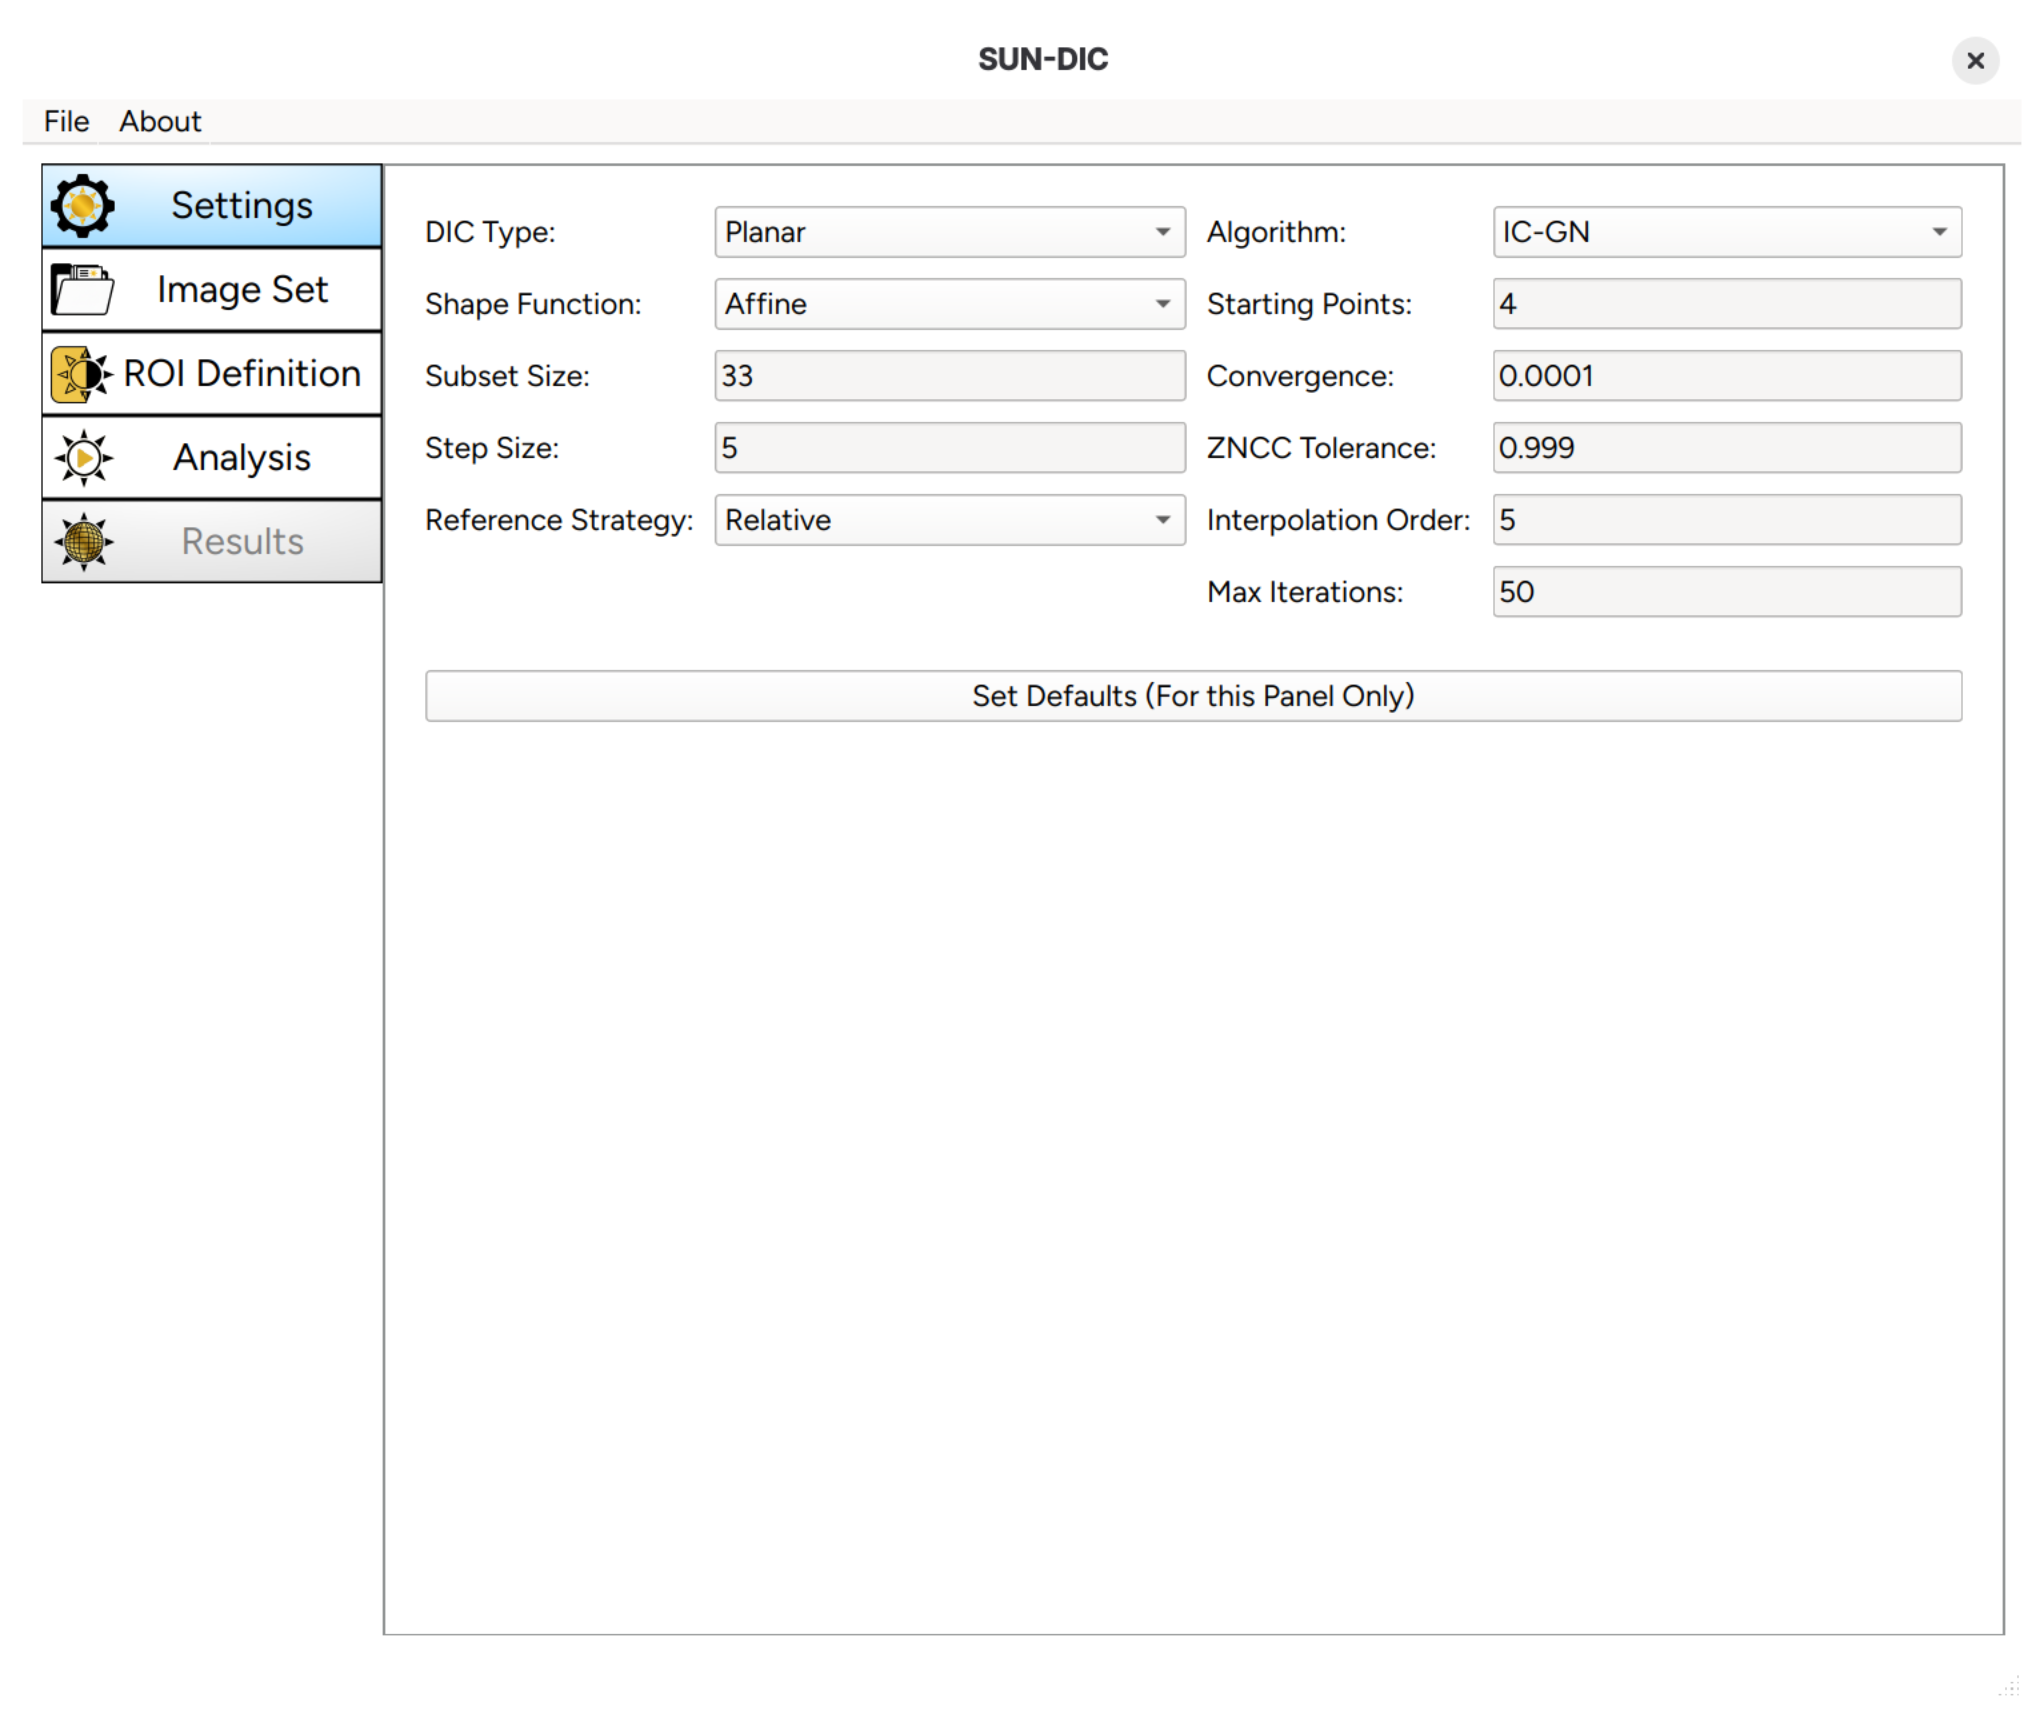
\includegraphics[width=0.85\textwidth]{../../screenshots/settings.png}
	\caption{Settings Tab. General SUN-DIC parameters are configured here.}
	\label{fig:gui_settings}
\end{figure}

\section{Image Set Tab}

The \codebf{Image Set} tab is used to define the image set that will be used during the DIC analysis. Click the \codebf{Select Directory} button to choose the folder containing the image sequence. This folder should contain only the image sequence, as all files in the directory will be considered. The selected folder path is displayed in the \codebf{Folder} field. Images are considered in natural sort order.

To define the image set, the first and last images in the range are specified using the \codebf{Start} and \codebf{End} fields, while the \codebf{Increment} field defines the spacing between images in the sequence. The \codebf{Set Max} button can be used to automatically set the \codebf{End} field to the last image in the folder. The default behaviour is to consider all images in the selected image folder. The selected images are displayed in the \codebf{Images} list.

The \textbf{Advanced Settings} area exposes two pre-processing parameters: Gaussian blur kernel size (for noise reduction) and the background cut-off value. The background cut-off is used to automatically detect dark regions (e.g.\ holes) that are treated as background and automatically excluded from the ROI. Subsets with mean intensity below the specified threshold value are ignored.

The \textbf{Set Defaults (For this Panel Only)} button may be used to restore factory defaults for this tab only without affecting other settings.

\begin{figure}[!hbtp]
	\centering
	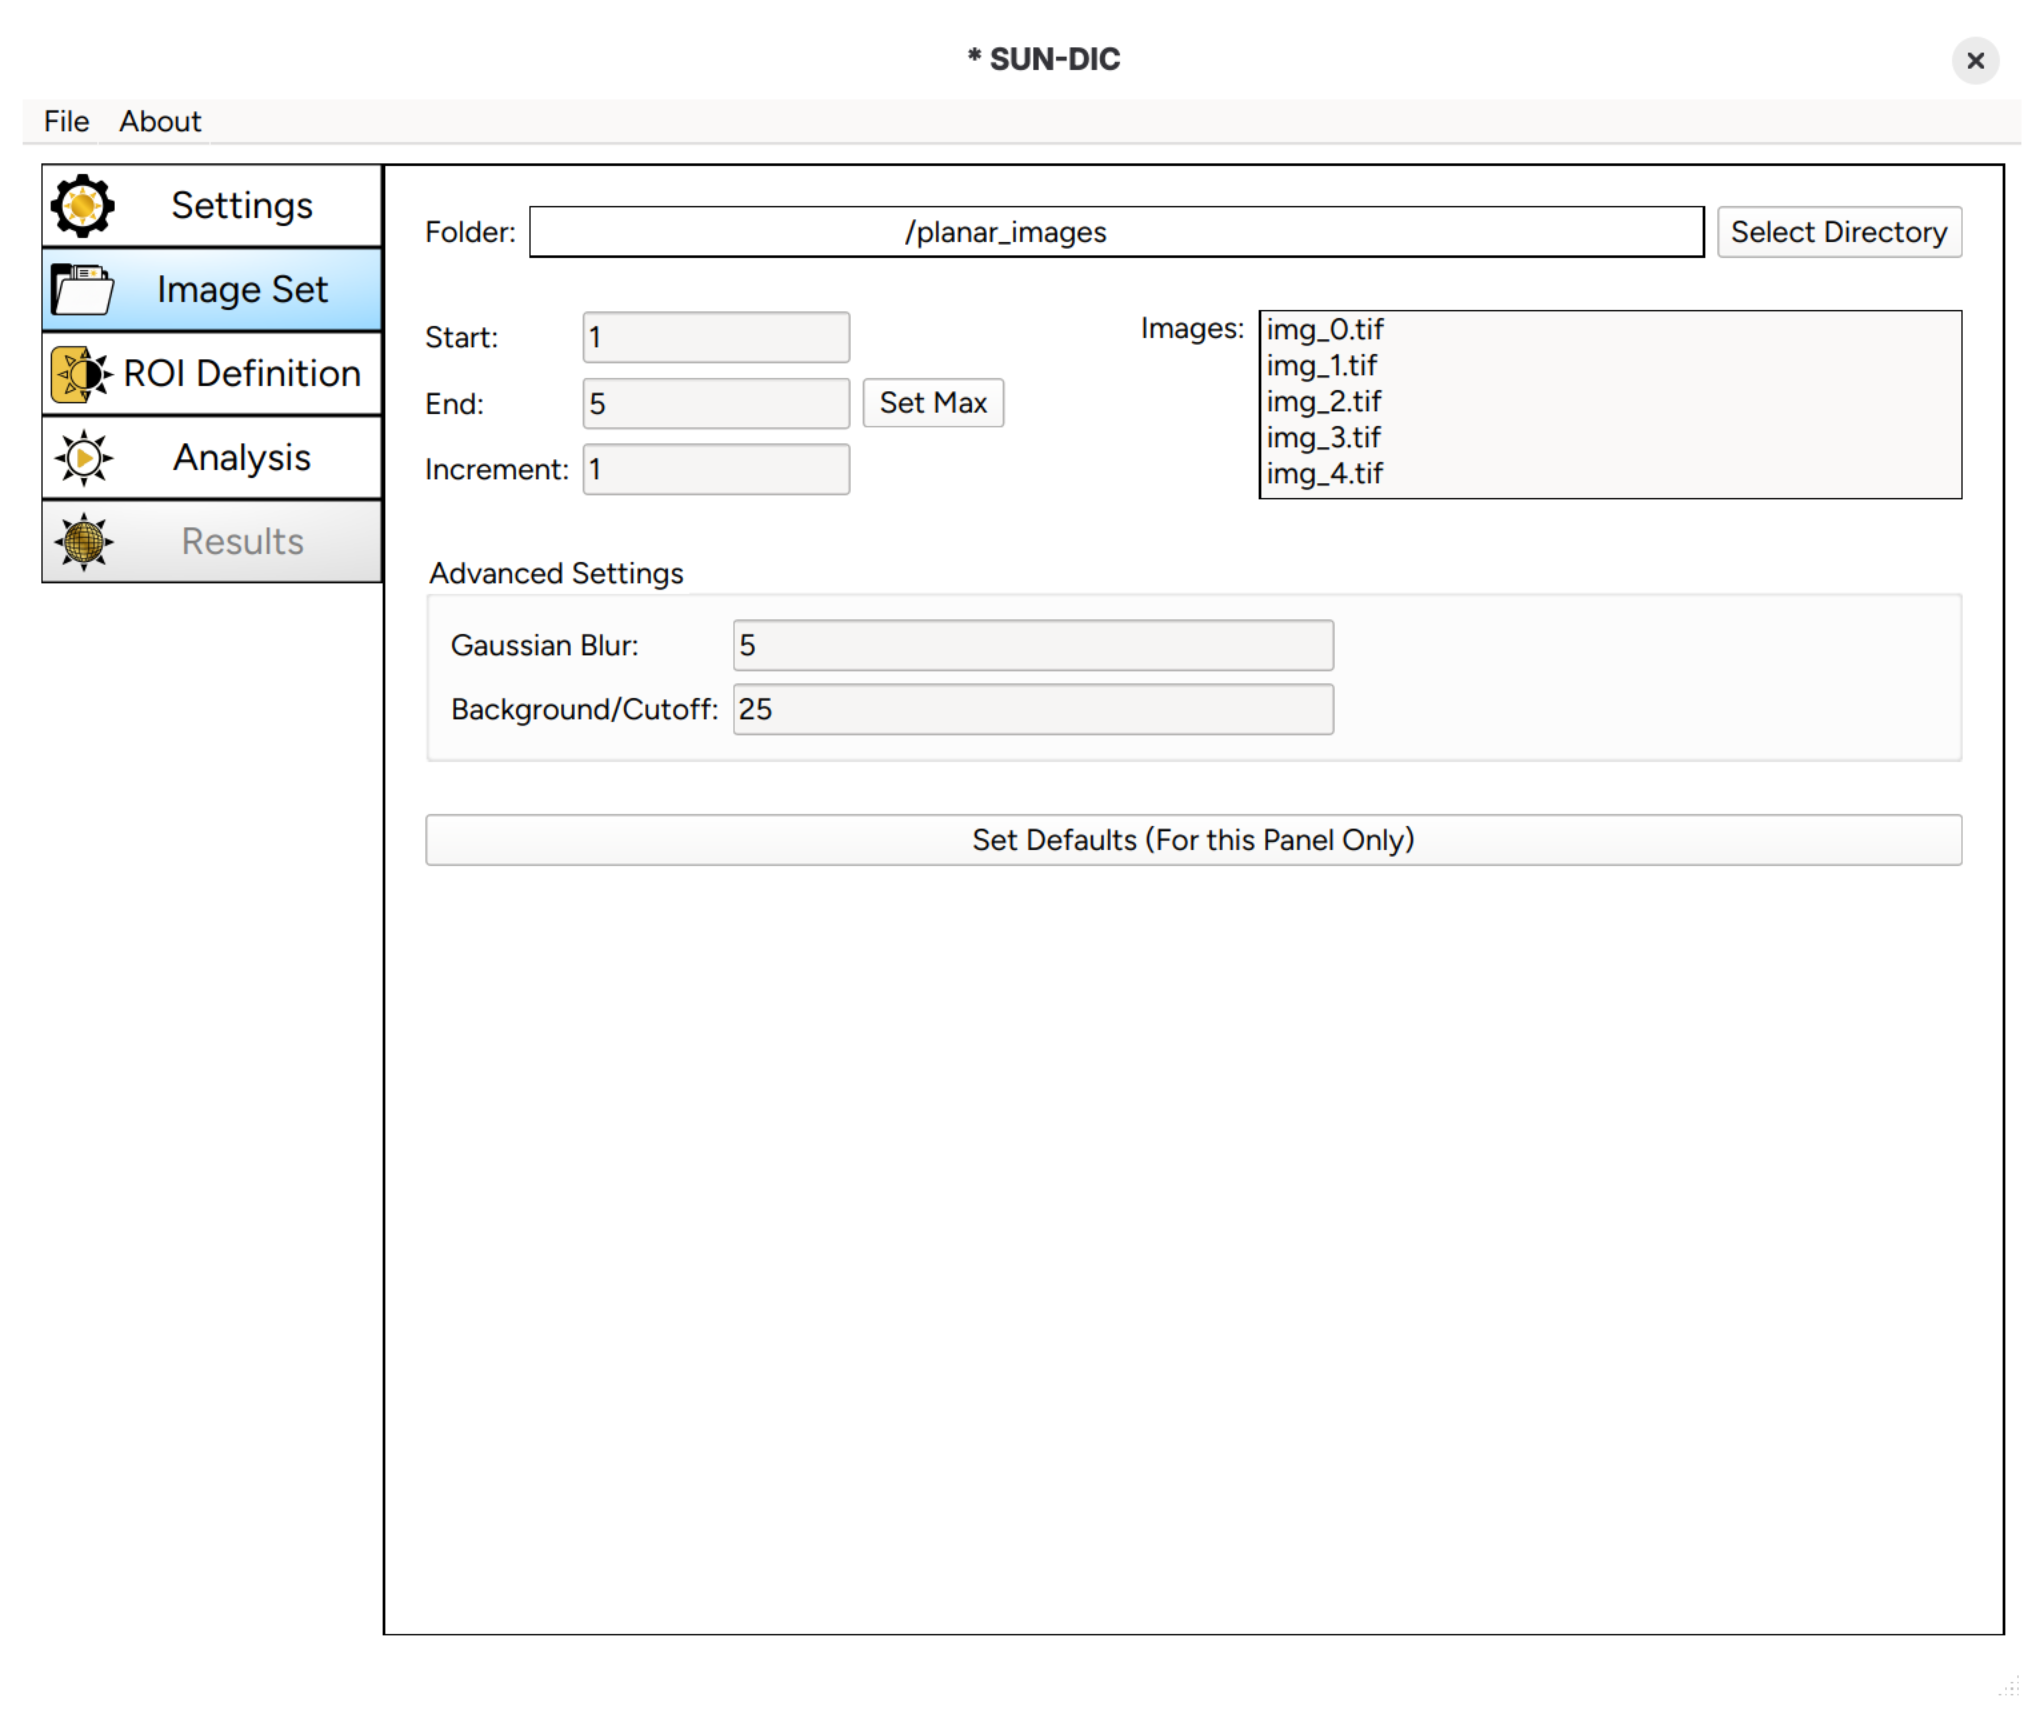
\includegraphics[width=0.85\textwidth]{../../screenshots/image_set.png}
	\caption{Image Set Tab. Select image folder, datum image, and target range.}
	\label{fig:gui_imageset}
\end{figure}

\section{ROI Definition Tab}

The \codebf{ROI Definition} tab is used to define and visualise the ROI. The datum image selected in the \codebf{Image Set} tab is displayed in an interactive viewer where the ROI is defined. The ROI is defined by clicking and dragging the mouse over the image to draw a rectangular region. It is shown as a red outline, and green markers indicate active subset centres so that coverage can be verified before running the analysis.

The four numeric fields (\codebf{Top Left x}, \codebf{Top Left y}, \codebf{Width}, \codebf{Height}) update automatically but may also be edited manually for precise control.

\newpage
\noindent
\textbf{Navigation controls:}
\begin{itemize}
	\item \textbf{Mouse wheel} -- Zoom in/out centered on the cursor.
	\item \textbf{Shift + left-drag} -- Pan the image.
	\item \textbf{Status bar} -- Displays the current cursor coordinates.
\end{itemize}

Specifying a binary mask is optional. Enable the \codebf{Use ROI binary mask} checkbox and select a mask file to exclude irregular regions from the analysis. The mask must be a single-channel binary image of the same size as the input images, where white indicates inclusion and black indicates exclusion.

\begin{figure}[!htbp]
	\centering
	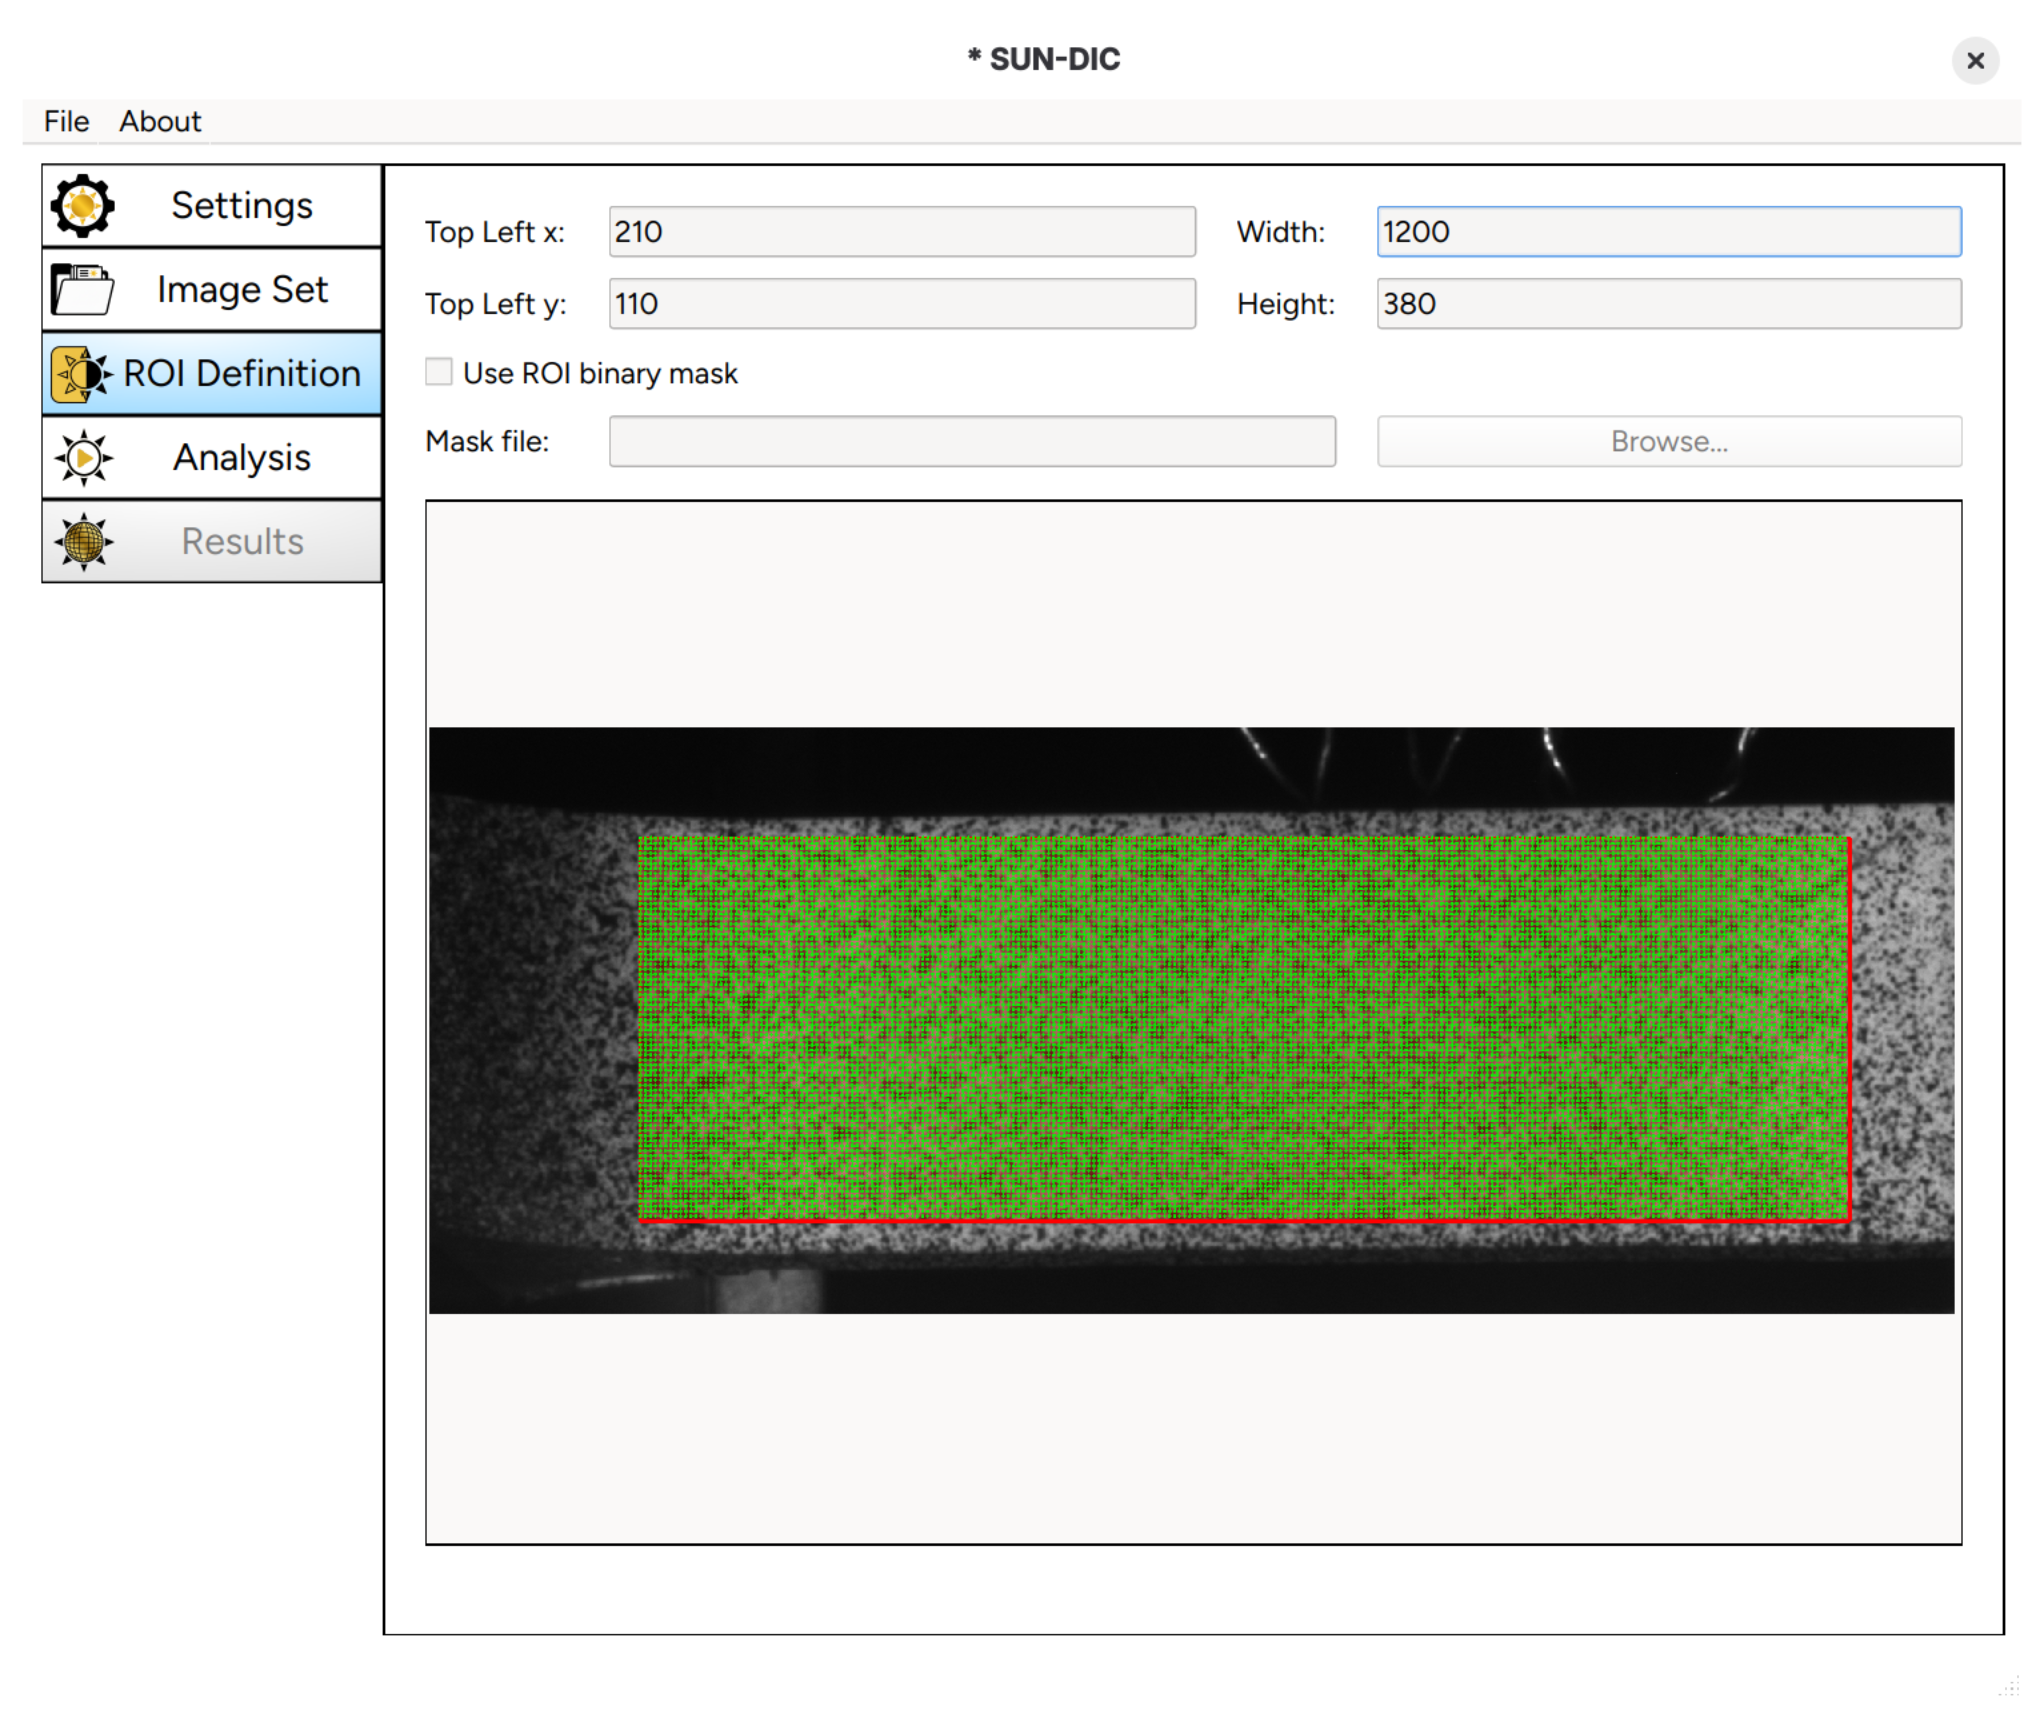
\includegraphics[width=0.85\textwidth]{../../screenshots/roi.png}
	\caption{ROI Definition Tab. Define the region of interest on the datum image.}
	\label{fig:gui_roi}
\end{figure}

\section{Analysis Tab}

The \codebf{Analysis} tab is used to perform the DIC analysis. Two runtime parameters can be configured in this tab:

\begin{itemize}
	\item \codebf{Debug Level} -- Controls verbosity of console output where 0 is no debug output, 1 corresponds to top-level output and 2 corresponds to per-iteration level output.  Note that debug output is limited when running the analysis in parallel.
	\item \codebf{CPU Count} -- The number of parallel worker processes to use during the analysis.
\end{itemize}

Click the \codebf{Start} button to begin the analysis. Live output is displayed in the output panel. The status indicator turns blue while running, green when complete, and red if the run is interrupted. Click the \codebf{Stop} button to abort execution.

Results are written to a binary \code{.sdic} file in the working directory. This file should not be saved inside the image directory, since all files in that directory are assumed to be image files during analysis.

\begin{figure}[htbp]
	\centering
	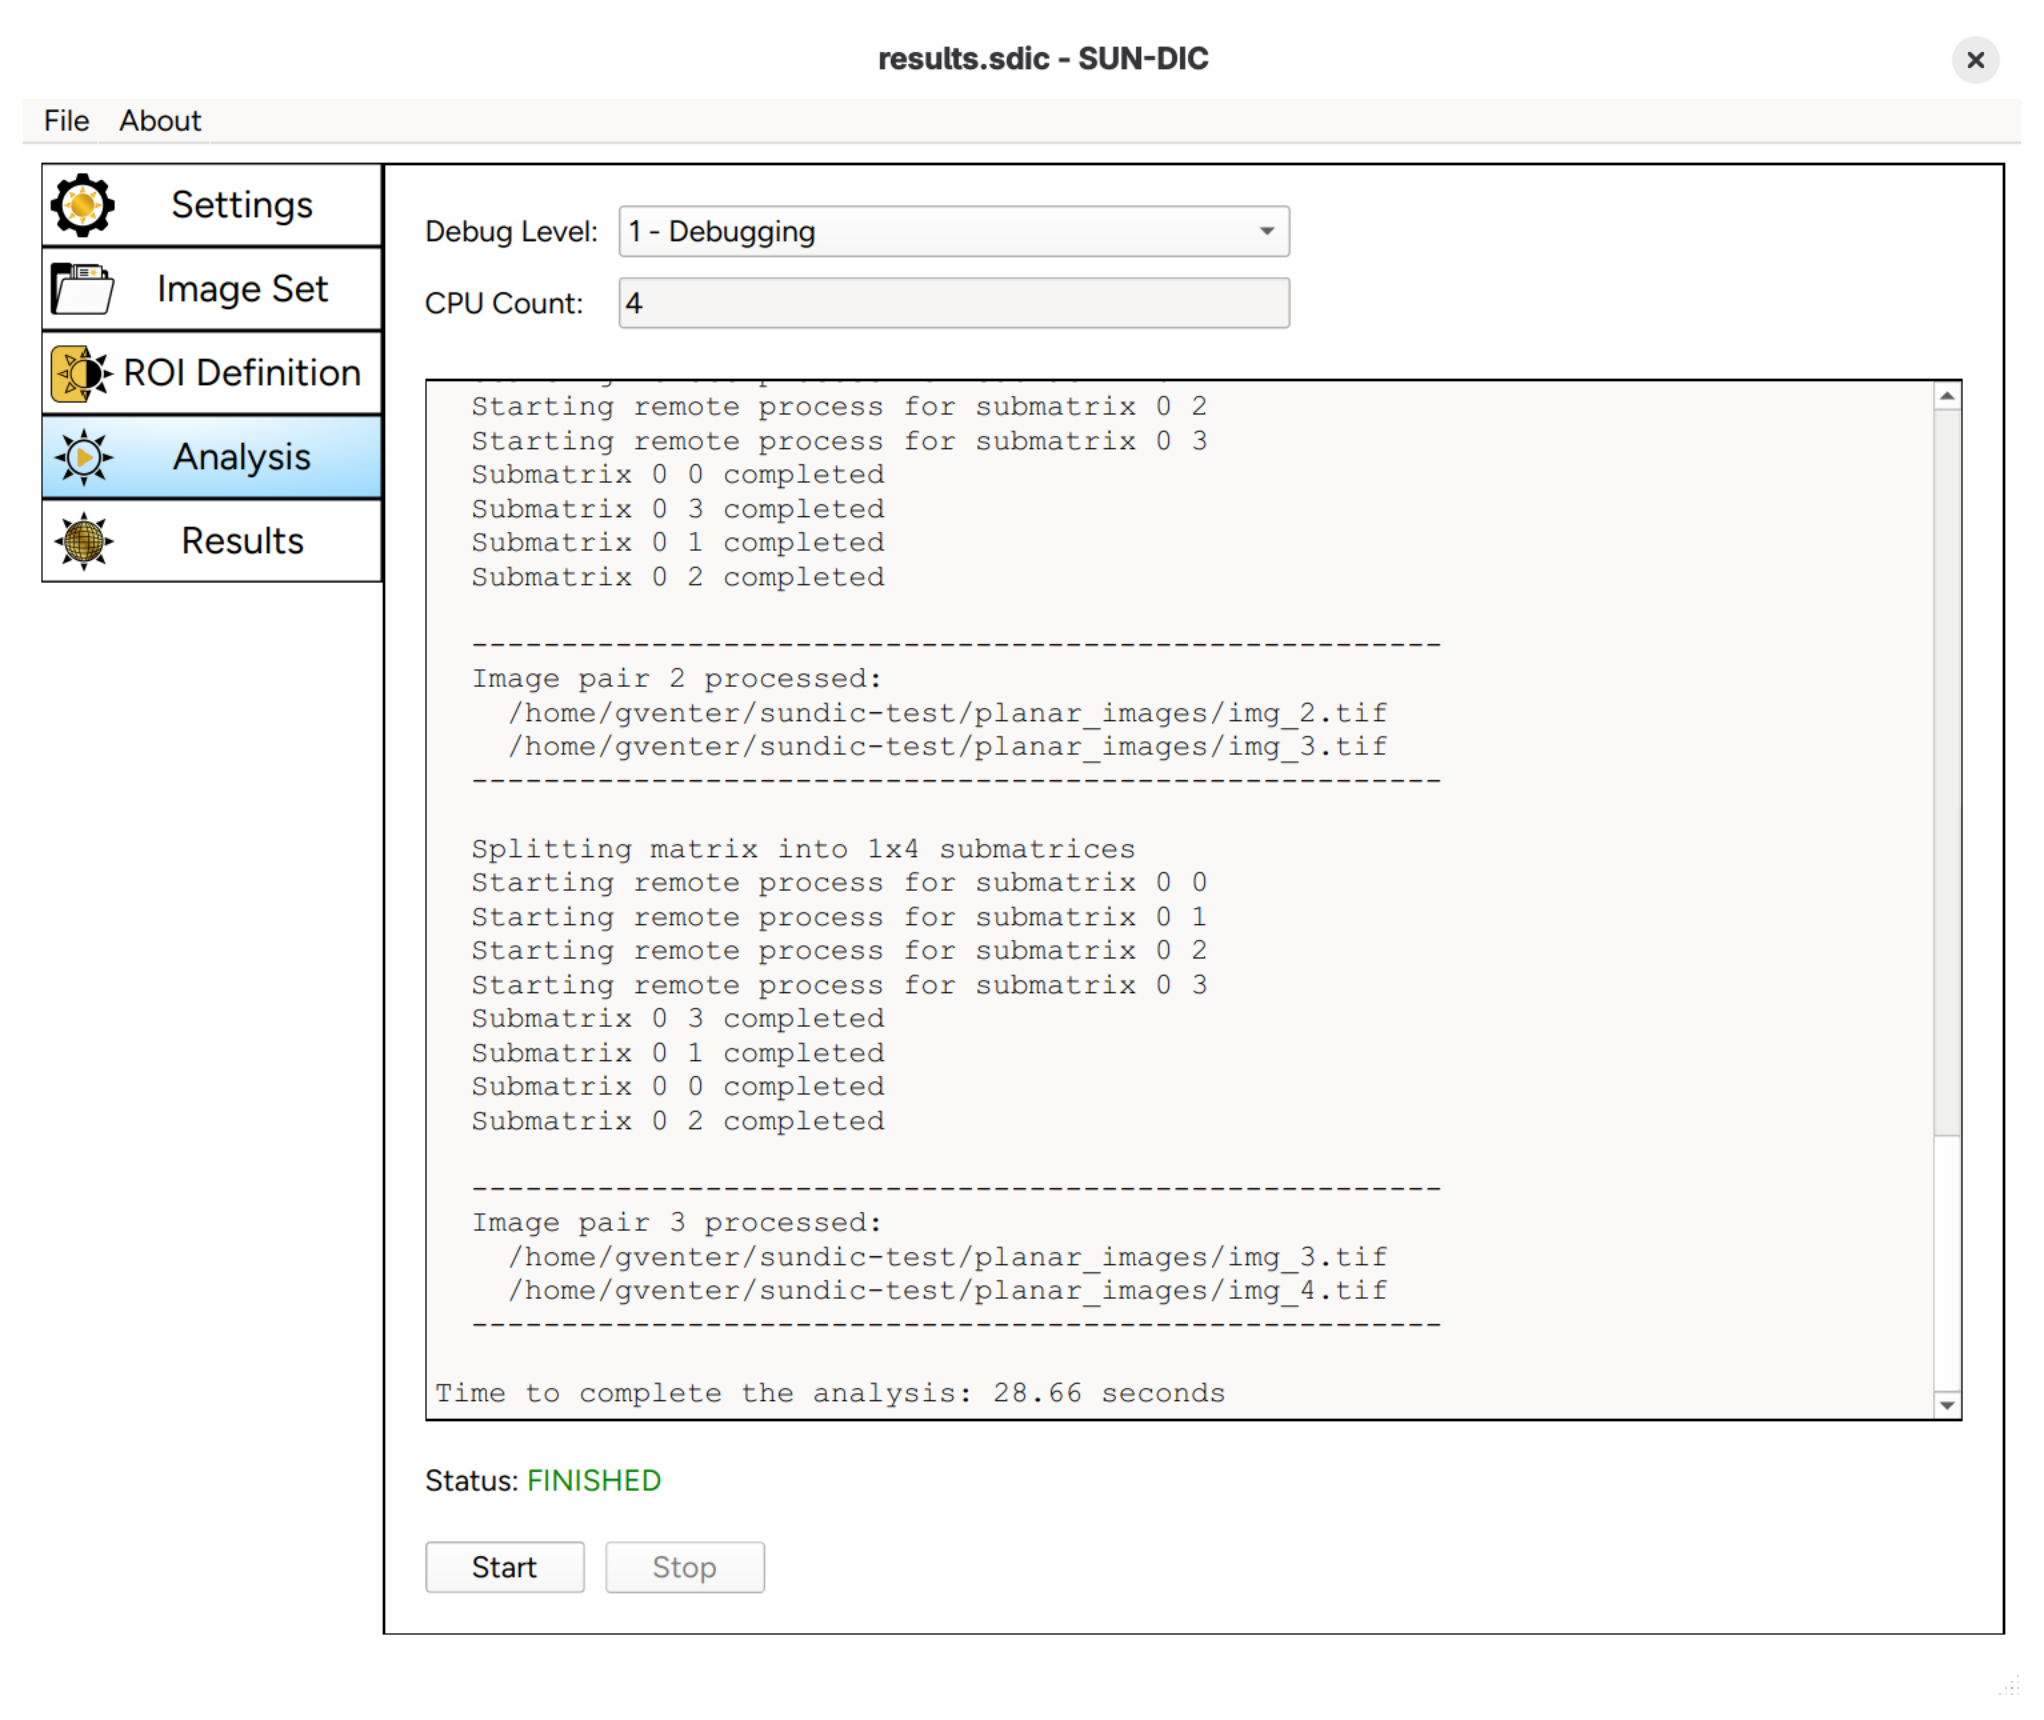
\includegraphics[width=0.85\textwidth]{../../screenshots/analyze.png}
	\caption{Analysis Tab. Run the DIC engine and monitor progress.}
	\label{fig:gui_analysis}
\end{figure}

\section{Results Tab}

The \codebf{Results} tab is used for post-processing the analysis results. The \codebf{Results} tab becomes active when there are results in the \code{.sdic} file, typically after the analysis is complete. Three view modes are available via the buttons at the top of the panel.

\begin{figure}[htbp]
	\centering
	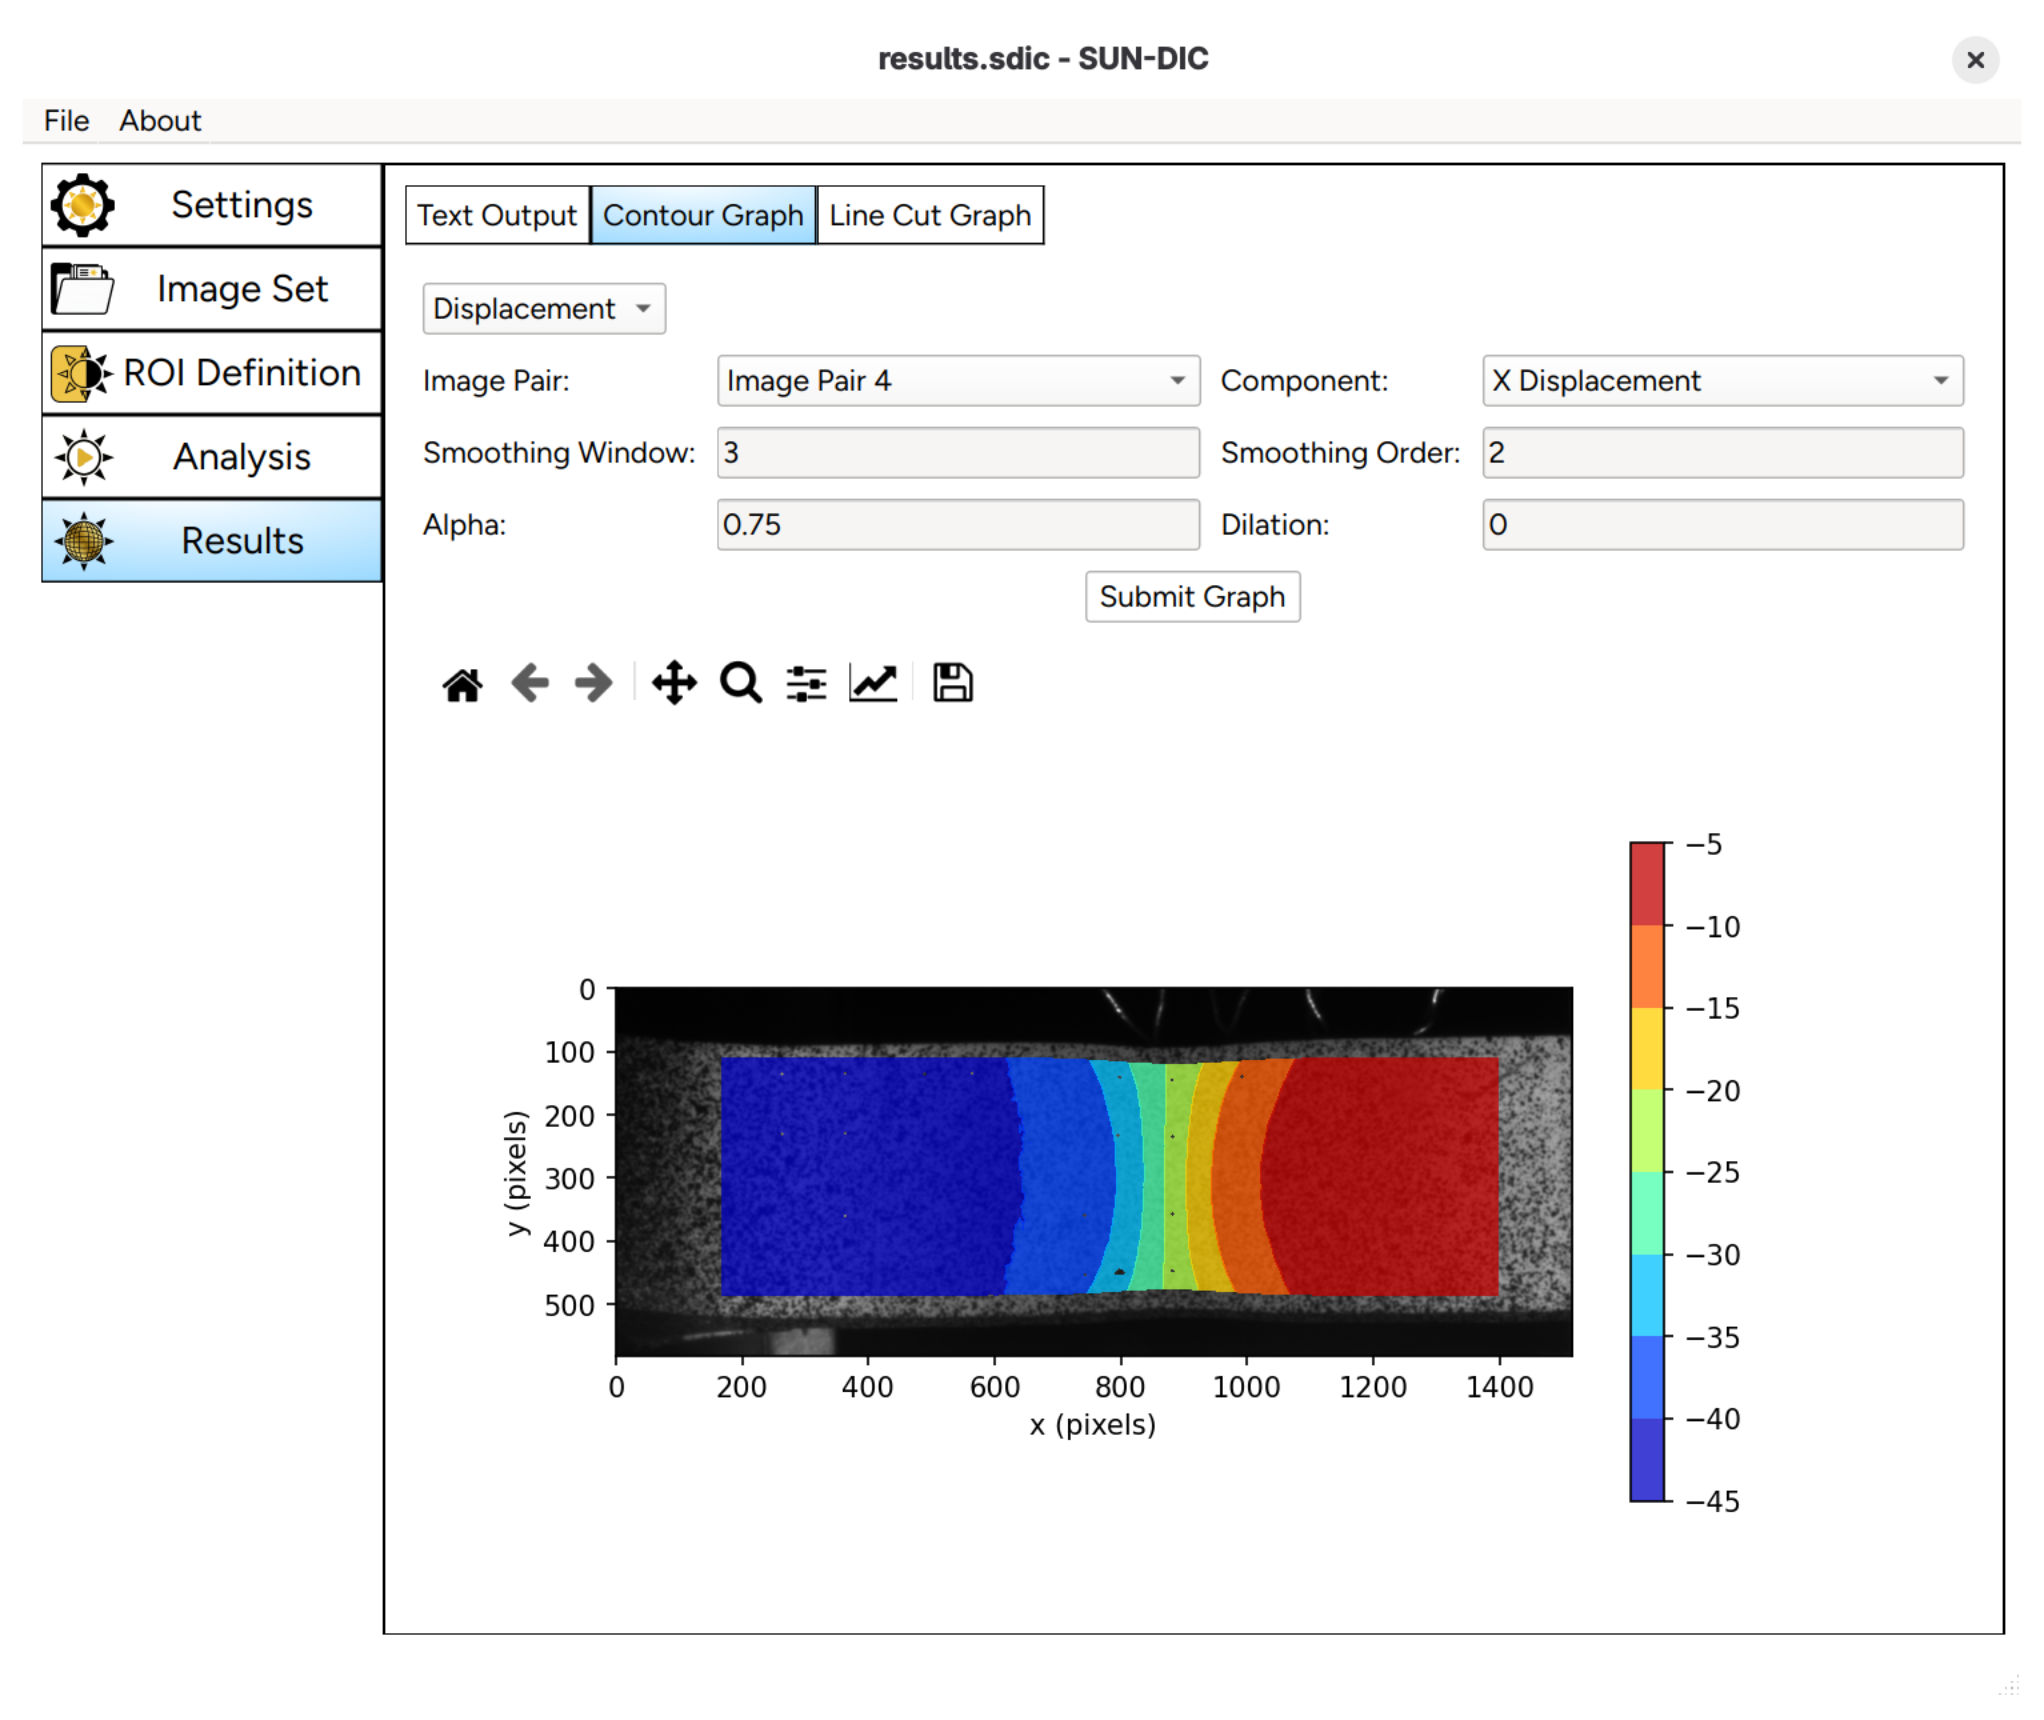
\includegraphics[width=0.85\textwidth]{../../screenshots/results.png}
	\caption{Results Tab. Contour plots, line cuts, and data export views.}
	\label{fig:gui_results}
\end{figure}

\newpage
\subsection{Contour Graph}

The \codebf{Contour Graph} panel is used to create contour plots of the computed field data over the specimen. This panel provides the following options:

\begin{itemize}
	\item \codebf{Results} -- Choose Displacement, Strain, or Correlation data to plot.
	\item \codebf{Image Pair} -- Select the image pair for post-processing.
	\item \codebf{Component} -- Select the field component: $u$ (X displacement), $v$ (Y displacement), displacement magnitude, $\varepsilon_x$, $\varepsilon_y$, $\varepsilon_{xy}$, or Von Mises strain $\varepsilon_\text{VM}$.
	\item \codebf{Smoothing Window / Order} -- Window size and polynomial order for Savitzky--Golay smoothing.
	\item \codebf{Alpha} -- Transparency of the contour overlay.
	\item \codebf{Dilation} -- Number of subsets to expand the exclusion mask, useful for edge cleaning.
\end{itemize}

Click the \textbf{Submit Graph} button to generate the plot.

\subsection{Line Cut Graph}

The \codebf{Line Cut Graph} panel is used to create two-dimensional line plots through the computed field data. A line-cut graph plots field values along one or more straight lines through the domain. This panel provides the following options:

\begin{itemize}
	\item \codebf{Results} -- Choose Displacement or Strain data to plot.
	\item \codebf{Image Pair} -- Select the image pair for post-processing.
	\item \codebf{Display Component} -- Select the field component: $u$ (X displacement), $v$ (Y displacement), displacement magnitude, $\varepsilon_x$, $\varepsilon_y$, $\varepsilon_{xy}$, or Von Mises strain $\varepsilon_\text{VM}$.
	\item \codebf{Cut Component} -- Axis along which cuts are taken (X or Y coordinate).
	\item \codebf{Cut Values} -- Comma-separated list of positions at which to make the cuts, e.g.\ \code{250, 300, 350}.
	\item \codebf{Smoothing Window / Order} -- Window size and polynomial order for Savitzky--Golay smoothing.
	\item \codebf{Dilation} -- Number of subsets to expand the exclusion mask, useful for edge cleaning.
	\item \codebf{Interpolate} -- Interpolate data onto a uniform grid before plotting. When this option is selected, the exact cut values are used. Otherwise, the nearest row or column of subset centres is used.
	\item \codebf{Grid Lines} -- Display grid lines on the graph.
\end{itemize}

Click the \textbf{Submit Graph} button to generate the plot.

\subsection{Text Output}

The \codebf{Text Output} panel is used to export the raw computed field data for external processing and provides the following options:

\begin{itemize}
	\item \codebf{Image Pair} -- Image pair to export.
	\item \codebf{Include Displacements / Strains} -- Select output fields to export.
	\item \codebf{Remove NaNs} -- Exclude failed or invalid subsets.
	\item \codebf{Smoothing Window / Order} -- Optional preprocessing before export. Uses a Savitzky--Golay filter to reduce noise in the exported data.
	\item \codebf{Dilation} -- Number of subsets to expand the exclusion mask, useful for edge cleaning.
\end{itemize}

Click the \textbf{Export Data} button to write the data to a \code{.csv} output file. The column structure matches the raw data format described in Section~\ref{sec:api}.

\section{Example Problem}

To run the example problem in the GUI, proceed as follows:

\begin{enumerate}
	\item Copy the example files to your working directory:
	
\begin{lstlisting}[language=bash]
copy-examples
\end{lstlisting}
	
	\textbf{This creates:}
	
	\begin{itemize}
		\item \code{test\_sundic.ipynb} -- Worked Python API example in Jupyter notebook format
		\item \code{settings.ini} -- Fully documented configuration file usable in both the GUI and API
		\item \code{planar\_images/} -- Sample TIFF image sequence for testing
	\end{itemize}
	
	\item Launch the GUI:
	
\begin{lstlisting}[language=bash]
sundic
\end{lstlisting}
	
	\item Import the \code{settings.ini} configuration via \textbf{File $\rightarrow$ Import Settings File}.
	
	\item Verify that settings, images, and ROI are correctly loaded. If the image files are not found, manually browse to the \code{planar\_images} folder.
	
	\item Run the analysis from the \textbf{Analysis} tab.
	
	\item Explore the results in the \textbf{Results} tab.
	
\end{enumerate}

You are encouraged to modify settings and rerun the analysis to explore different configurations and effects.

% ─────────────────────────────────────────────────────────────────────────────
\chapter{Python API Workflow and Example}
\label{sec:api}
% ─────────────────────────────────────────────────────────────────────────────

\section{Setup}

Start by copying the example problem to your working directory by issuing the
\code{copy-examples} command from a terminal after activating your virtual
environment. After running \code{copy-examples}, the working directory will
contain:

\begin{itemize}
	\item \code{settings.ini} -- Example configuration file
	\item \code{planar\_images/} -- Five sample TIFF images
	\item \code{test\_sundic.ipynb} -- Jupyter notebook containing a complete worked example
\end{itemize}

The Jupyter notebook is the recommended starting point for new users because it
demonstrates every step described in this chapter with live output and
visualisation. The API can also be used directly from a standard Python
\code{.py} script.

If you intend to use the provided notebook, remember to install the optional Jupyter
dependencies using:

\begin{lstlisting}[language=bash]
pip install ./SUN-DIC[jupyter]
\end{lstlisting}

\section{API Module Overview}

Most users will interact with only three modules:

\begin{itemize}
	\item \code{sundic.settings} -- Reading, writing, and managing analysis settings.
	\item \code{sundic.sundic} -- Running the DIC analysis.
	\item \code{sundic.post\_process} -- Visualisation, export, and access to computed results.
\end{itemize}

\noindent
The typical workflow is:

\begin{enumerate}
	\item Load a \code{settings.ini} file.
	\item Run the DIC analysis.
	\item Open the resulting \code{.sdic} file for post-processing.
	\item Generate plots, export data, or access NumPy arrays directly.
\end{enumerate}

The API follows a two-phase workflow. During the first phase, the DIC analysis reads the configuration and image sequence and writes all results to a binary \code{.sdic} file.

During the second phase, post-processing functions read the \code{.sdic} file
on demand to generate displacement fields, strain fields, contour plots,
line-cut graphs, correlation-quality plots, and exported data files.

Because all results are stored in the \code{.sdic} file, the computationally
expensive DIC analysis only needs to be performed once. Post-processing
operations can then be repeated with different settings without rerunning the
analysis.

\section{Running an Analysis}

Settings are loaded from a \code{settings.ini} file and passed directly to the
analysis function along with a name for the output file. The fully documented
\code{settings.ini} provided with the example problem is a good starting point
for creating a custom configuration file for your own analysis.

The \code{Settings} class implements a custom string representation, allowing the current configuration to be printed directly. The following listing reads the provided
\code{settings.ini} file, prints the configuration to the screen, and then
submits the DIC analysis using the \code{planarDICLocal} function.


\begin{lstlisting}
import sundic.sundic as sdic
import sundic.settings as sdset

settings = sdset.Settings.fromSettingsFile('settings.ini')
print(settings)

sdic.planarDICLocal(settings, 'results.sdic')
\end{lstlisting}

Debug output is printed to the console as each image pair is processed.  All raw results and the settings snapshot are stored in the specified \code{results.sdic} file.  This is a SUN-DIC specific binary file that can also be opened in the GUI for post-processing.

The \code{planarDICLocal} function has an optional argument named \code{externalRay} that can be set to \code{True} if a Ray server was started separately from the API run.  This is useful when running a number of DIC analyses in a loop where an external Ray server reduces the overhead of starting and stopping the server each time an analysis is performed.  The call to \code{planarDICLocal} would then look as follows:

\begin{lstlisting}
sdic.planarDICLocal(settings, 'results.sdic', externalRay=True)
\end{lstlisting}

The external Ray server is typically started from the terminal using the following command.  There are however more advanced options available for starting a Ray server, please refer to the Ray documentation.

\begin{lstlisting}
ray start --head
\end{lstlisting}


\section{Post-Processing}

All post-processing functions live in \code{sundic.post\_process} and accept the
output file path together with an image-pair index (\code{imgPair}).
Use \code{0} for the first pair or \code{-1} for the last. Throughout this chapter, the parameter \code{imgPair} identifies the image pair to process. Image pairs are numbered starting from zero. A value of \code{imgPair = 0} corresponds to the first image pair in the analysis, while \code{imgPair = -1} refers to the last available image pair.

\subsection{Smoothing}

Displacement and strain plot and data access functions all accept a \code{smoothWindow} (odd integer) and a \code{smoothOrder} (int) parameter to apply Savitzky-Golay smoothing before plotting.  For the displacement data, the smoothing is optional, while for the strain data it is required.  Strain calculations always apply smoothing with the window size defaulting to 9 but this value should be increased for noisier data.


\subsection{Contour Plots}

The following listing will produce contour graphs for X and Y displacement components, followed by contour graphs of the X and Von Mises strain components.

\begin{lstlisting}
import sundic.post_process as sdpp

# Displacement contour plots
sdpp.plotDispContour('results.sdic', -1, dispComp=sdpp.DispComp.X_DISP)
sdpp.plotDispContour('results.sdic', -1, dispComp=sdpp.DispComp.Y_DISP)

# Strain contour plots
sdpp.plotStrainContour('results.sdic', -1,
                       strainComp=sdpp.StrainComp.X_STRAIN)
sdpp.plotStrainContour('results.sdic', -1,
                       strainComp=sdpp.StrainComp.VM_STRAIN)
\end{lstlisting}

\newpage
\noindent
A complete list of arguments for these contour plot functions are summarized below:

\begin{lstlisting}
# Required Parameters:
# ------------------------------------------------------------------
# resultsFile (str) : the binary results file name to read
# imgPair (int)     : the zero based image pair ID to process
# 
# Optional Parameters:
# ------------------------------------------------------------------
# alpha (float)     : the transparency of the contour plot
#                     (Default is 0.75 -> 75% opaque)
# plotImage (bool)  : whether to plot the underlying image
#                     (Default is True -> plot the underlying image)
# showPlot (bool)   : whether to show the plot here
#                     (Default is True -> show the plot)
# fileName (str)    : the file name to save the plot to if 
#                     required
#                     (Default is '' -> No file saved)
# smoothWindow (int): the size of the smoothing window
#                     this is the number of surrounding subSets to 
#                     consider in the smoothing 
#                     (Default=0 -> no smoothing)
# smoothOrder (int) : the order of the smoothing polynomial 
#                     (Default=2 -> quadratic smoothing)
# dilation (int)    : the number of subsets to dilate the mask 
#                     around automatically detected features (eg holes) 
#                     where the results may be of poor quality 
#                     (Default = 0  -> no dilation)
# maxValue (float)  : the maximum value to plot
#                     (Default is None -> auto scale)
# minValue (float)  : the minimum value to plot
#                     (Default is None -> auto scale)
\end{lstlisting}

For \code{plotDispContour} there is an additional optional parameter \code{dispComp} to identify the displacement component to plot.  Available \code{dispComp} values are \code{X\_DISP}, \code{Y\_DISP}, and \code{DISP\_MAG}.

\begin{lstlisting}
# dispComp (int)    : the displacement component to plot
#                     (Default is sdpp.DispComp.MAG -> Magnitude)
\end{lstlisting}


For \code{plotStrainContour} the corresponding parameter to identify the strain component to plot is \code{strainComp} and available \code{strainComp} values are  \code{X\_STRAIN}, \code{Y\_STRAIN}, \code{SHEAR\_STRAIN}, and \code{VM\_STRAIN}.

\begin{lstlisting}
# strainComp (int)  : the strain component to plot
#                     (Default is sdpp.StrainComp.VM_STRAIN)
\end{lstlisting}


\subsection{Correlation Quality Plot}

A filled contour map of the ZNCC correlation quality field can be plotted to identify
subsets that converged poorly:

\begin{lstlisting}
import sundic.post_process as sdpp

sdpp.plotZNCCContour('results.sdic', -1)
\end{lstlisting}

ZNCC ranges from $-1$ to $1$, with $1$ indicating a perfect match.
Values close to $1$ across the domain indicate a reliable analysis.  Low or negative
values flag problematic regions (poor speckle, occlusion, large out-of-plane motion).  A complete list of parameters for the \code{plotZNCCContour} function are summarized below.

\begin{lstlisting}
# Required Parameters:
# ------------------------------------------------------------------
# resultsFile (str) : the binary results file name to read
# imgPair (int)     : the zero based image pair ID to process
# 
# Optional Parameters:
# ------------------------------------------------------------------
# alpha (float)     : the transparency of the contour plot
#                     (Default is 0.75 -> 75% opaque)
# plotImage (bool)  : whether to plot the underlying image
#                     (Default is True -> Plot the underlying image)
# showPlot (bool)   : whether to show the plot here
#                     (Default is True -> Show the plot)
# fileName (str)    : the file name to save the plot to if 
#                     required
#                     (Default is '' -> No file saved)
# maxValue (float)  : the maximum value to plot
#                     (Default is None -> auto scale)
# minValue (float)  : the minimum value to plot
#                     (Default is None -> auto scale)
\end{lstlisting}


\subsection{Line Cuts}

A line-cut graph plots field values along one or more straight lines through the domain. The \code{plotDispCutLine} and \code{plotStrainCutLine} functions extract displacement or strain values along one or more straight cuts through the image.  The listing below shows how to generate a displacement line-cut graph for the X  displacement with cuts at 250, 300 and 350 pixels along the Y coordinate.  This results in a 2D graph with three lines.  The second function call in the listing generates a line-cut graph for the Von Mises strain with cuts at 500 and 700 pixels along the X coordinate. A 2D graph with two lines will be produced.

\newpage
\begin{lstlisting}
import sundic.post_process as sdpp

# Line cut through the displacement field at fixed Y positions
sdpp.plotDispCutLine('results.sdic', -1,
	dispComp=sdpp.DispComp.X_DISP,
	cutComp=sdpp.CompID.YCoordID,
	cutValues=[250, 300, 350])
	
# Von Mises strain along fixed X positions
sdpp.plotStrainCutLine('results.sdic', -1,
	strainComp=sdpp.StrainComp.VM_STRAIN,
	cutComp=sdpp.CompID.XCoordID,
	cutValues=[500, 700])
\end{lstlisting}

A complete list of parameters for the \code{plotDispCutLine}  and \code{plotStrainCutLine} functions are summarized below.

\begin{lstlisting}
# Required Parameters:
# ------------------------------------------------------------------
# resultsFile (str) : the binary results file name to read
# imgPair (int)     : the zero based image pair ID to process
# 
# Optional Parameters:
# ------------------------------------------------------------------
# cutComp (int)     : the component to cut through
#                     (Default is sdpp.CompID.XCoordID -> X coordinate)
# cutValues (list)  : the values to cut through
#                     (Default is None -> No cuts)
# gridLines (bool)  : whether to plot grid lines
#                     (Default is True -> Plot grid lines)
# showPlot (bool)   : whether to show the plot here
#                     (Default is True -> Show the plot)
# fileName (str)    : the file name to save the plot to
#                     (Default is '' -> No file saved)
# smoothWindow (int): the size of the smoothing window
#                     this is the number of surrounding subSets to 
#                     consider in the smoothing
#                     (Default is 0 -> no smoothing)
# smoothOrder (int) : the order of the smoothing polynomial
#                     (Default is 2 -> quadratic smoothing)
# dilation (int)    : the number of subsets to dilate the mask 
#                     around automatically detected features (eg holes) 
#                     where the results may be of poor quality 
#                     (Default = 0  -> no dilation)
# interpolate (bool): whether to interpolate the data
#                     (Default is False -> no interpolation)
# -----------------------------------------------------------
\end{lstlisting}

\newpage
As for the contour plots, there is an additional optional parameter \code{dispComp} to identify the displacement component to plot when calling \code{plotDispCutLine}.  Available \code{dispComp} values are \code{X\_DISP}, \code{Y\_DISP}, and \code{DISP\_MAG}.

\begin{lstlisting}
# dispComp (int)    : the displacement component to plot
#                     (Default is sdpp.DispComp.MAG -> Magnitude)
\end{lstlisting}

For \code{plotStrainCutLine} the corresponding parameter to identify the strain component to plot is \code{strainComp} and available \code{strainComp} values are  \code{X\_STRAIN}, \code{Y\_STRAIN}, \code{SHEAR\_STRAIN}, and \code{VM\_STRAIN}.

\begin{lstlisting}
# strainComp (int)  : the strain component to plot
#                     (Default is sdpp.StrainComp.VM_STRAIN)
\end{lstlisting}

\subsection{Accessing Raw Data}

For custom analysis or export, the displacement and strain arrays can be retrieved
directly as \code{NumPy} arrays.  Each row corresponds to one subset point and missing points carry \code{NaN} values that can be filtered out with a standard \code{NumPy} mask.  The following listing first retrieves the displacement data and then the strain data.

\begin{lstlisting}
import sundic.post_process as sdpp

# Get raw displacement data for the last image pair
disp, nRows, nCols    = sdpp.getDisplacements('results.sdic', -1)

# Get raw strain data for the last image pair
strains, nRows, nCols = sdpp.getStrains('results.sdic', -1)
\end{lstlisting}

\noindent
The column layout for the displacement data is as follows:

\begin{lstlisting}
| X Coord | Y Coord | Z Coord | X Disp | Y Disp | Z Disp | Magnitude |
\end{lstlisting}

\noindent
The column layout for the strain data is as follows:

\begin{lstlisting}
|X Coord|Y Coord| Z Coord | X Strain | Y Strain | XY Strain | VM Strain |
\end{lstlisting}

\newpage
A complete list of parameters for the \code{getDisplacements}  and \code{getStrains} functions are summarized below.

\begin{lstlisting}
# Required Parameters:
# ------------------------------------------------------------------
# resultsFile (str) : the binary results file name to read
# imgPair (int)     : the zero based image pair ID to process
# 
# Optional Parameters:
# ------------------------------------------------------------------
# smoothWindow (int): the size of the smoothing window
#                     this is the number of surrounding subSets to 
#                     consider in the smoothing 
#                     (Default is 0 -> no smoothing for displacements
#                                 9 -> smoothing for strains)
# smoothOrder (int) : the order of the smoothing polynomial 
#                     (Default is 2 -> quadratic smoothing)
# dilation (int)    : the number of subsets to dilate the mask 
#                     around automatically detected features (eg holes) 
#                     where the results may be of poor quality 
#                     (Default is 0  -> no dilation)
#
# Returns:
# --------
# results: the displacement/strain results with the columns as outlined 
#          above
# nRows  : the number of subset rows in the image
# nCols  : the number of subset columns in the image
\end{lstlisting}
% ─────────────────────────────────────────────────────────────────────────────
\chapter{Theory}
\label{sec:theory}
% ─────────────────────────────────────────────────────────────────────────────

SUN-DIC implements local (subset-based) Digital Image Correlation
\citep{Sutton2009, Pan2018}, in which the image is divided into small overlapping
subsets that are independently tracked from a reference image to a deformed image.
The sections below provide a short summary of some of the key algorithmic components implemented in SUN-DIC. A good high level overview of DIC is provided by \href{https://digitalimagecorrelation.org/}{A practical guide to DIC}, while many excellent textbooks and academic papers are available for further reading.

\begin{grayquote}
	The purpose of this chapter is to provide a brief overview of the algorithms implemented in SUN-DIC. It is not intended to be a comprehensive introduction to Digital Image Correlation. Readers interested in detailed derivations and theoretical background are encouraged to consult the references cited throughout this chapter.
\end{grayquote}

% ─────────────────────────────────────────────────────────────────────────────
\section{The DIC Problem}

Let $f(\mathbf{x})$ be the intensity at pixel $\mathbf{x} = (x, y)$ in the reference
image and $g(\mathbf{x}')$ the intensity at the corresponding location in the deformed
image. A subset $S$ centred at $\mathbf{x}_0$ in the reference image is mapped to the
deformed image by a warp function $\mathcal{W}(\boldsymbol{\xi};\,\mathbf{p})$,
where $\boldsymbol{\xi} = (\xi,\eta)$ are local coordinates measured relative to the
subset centre and $\mathbf{p}$ is the vector of deformation parameters
(see Section~\ref{sec:shape}).

The goal of the optimisation is to determine the deformation parameters $\mathbf{p}$
that best align the reference subset with its counterpart in the deformed image by
minimising a correlation cost function.

% ─────────────────────────────────────────────────────────────────────────────
\section{Correlation Criterion}
\label{sec:znssd}

Many correlation criteria have been proposed in the DIC literature. SUN-DIC uses the
Zero-Mean Normalised Sum of Squared Differences (ZNSSD) criterion to determine the
optimal deformation parameters $\mathbf{p}$.  The ZNSSD criterion provides robustness to illumination changes by normalising intensity values within each subset:

\begin{equation}
	\label{eqn:znssd}
	C_\text{ZNSSD}(\mathbf{p}) =
	\sum_{\boldsymbol{\xi} \in S}
	\left[
	\frac{f(\mathbf{x}_0+\boldsymbol{\xi}) - \bar{f}}{\Delta f}
	-
	\frac{g\!\left(\mathcal{W}(\boldsymbol{\xi};\mathbf{p})\right) - \bar{g}}{\Delta g}
	\right]^2
\end{equation}
where $\bar{f}$ and $\bar{g}$ are the mean intensities of the reference and deformed
subsets, and

\begin{equation}
	\Delta f = \sqrt{\sum_{\boldsymbol{\xi} \in S}
		\bigl(f(\mathbf{x}_0+\boldsymbol{\xi}) - \bar{f}\bigr)^2},
	\qquad
	\Delta g = \sqrt{\sum_{\boldsymbol{\xi} \in S}
		\bigl(g\bigl(\mathcal{W}(\boldsymbol{\xi};\mathbf{p})\bigr) - \bar{g}\bigr)^2}
\end{equation}
are the $L_2$ norms of the zero-mean subsets. ZNSSD is insensitive to uniform changes in illumination offset and scale.

The closely related Zero-Mean Normalised Cross-Correlation (ZNCC) is related to ZNSSD by \citep{Pan2013a}:

\begin{equation}
	\label{eqn:zncc}
	\text{ZNCC} = 1 - \tfrac{1}{2}\,C_\text{ZNSSD}
\end{equation}

The ZNCC value ranges from $-1$ to $1$, where a value of $1$ indicates a perfect match between the reference and deformed subsets. SUN-DIC uses ZNCC as an optional convergence criterion via the \code{NZCCThreshold} parameter.

% ─────────────────────────────────────────────────────────────────────────────
\section{Subpixel Interpolation}

Deformation rarely produces integer-pixel shifts, so the deformed subset intensities
must be evaluated at non-integer pixel locations at every optimisation iteration.
Accurate subpixel interpolation is essential for measurement accuracy
\citep{Schreier2000}.

SUN-DIC uses bicubic (\code{InterpolationOrder=3}) or biquintic (\code{InterpolationOrder=5}) interpolation \citep{fast_interp}. Fifth-order interpolation is marginally more accurate, while third-order interpolation is generally more numerically robust and is recommended for most applications.

% ─────────────────────────────────────────────────────────────────────────────
\section{Shape Functions}
\label{sec:shape}

The mapping between the reference and deformed subsets is described by a shape function that approximates the local deformation within each subset. SUN-DIC supports both affine and quadratic shape functions.

\subsection{Affine Shape Functions (6~DOF)}

The affine warp uses six deformation parameters and is written in homogeneous matrix form \citep{Gao2015}:

\begin{equation}
	\label{eqn:affine}
	\mathcal{W}(\boldsymbol{\xi};\,\mathbf{p})
	=
	\begin{bmatrix}
		1+u_x & u_y   & u \\
		v_x   & 1+v_y & v \\
		0     & 0     & 1
	\end{bmatrix}
	\begin{pmatrix} \xi \\ \eta \\ 1 \end{pmatrix}
\end{equation}
with $\mathbf{p} = (u,\,u_x,\,u_y,\,v,\,v_x,\,v_y)^T$, where $(u, v)$ are the in-plane translations and $(u_x,\,u_y,\,v_x,\,v_y)$ are first-order displacement gradients that capture uniform stretching, rotation, and shear within the subset. Figure~\ref{fig:affine_theory} illustrates the transformation.

\begin{figure}[!hbt]
	\centering
	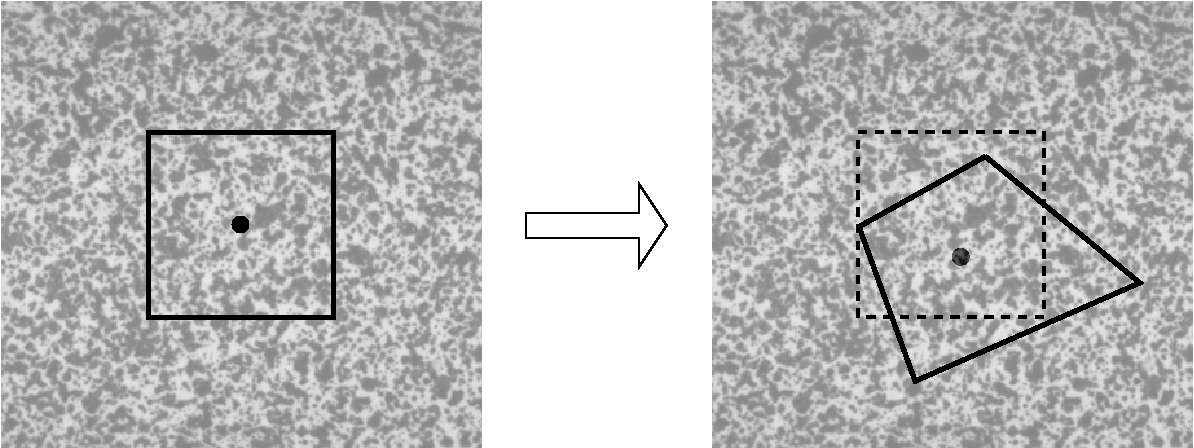
\includegraphics[width=9cm]{figures/affine-crop.pdf}
	\caption{Affine transformation from reference (left) to deformed (right) subset.}
	\label{fig:affine_theory}
\end{figure}

\subsection{Quadratic Shape Functions (12~DOF)}

The quadratic warp adds second-order terms, increasing the parameter vector to

\[
\mathbf{p} = (u,\,u_x,\,u_y,\,u_{xx},\,u_{xy},\,u_{yy},\,
v,\,v_x,\,v_y,\,v_{xx},\,v_{xy},\,v_{yy})^T.
\]

This model can better represent non-uniform deformation, bending, and large strain gradients. However, the additional degrees of freedom increase sensitivity to noise and generally require larger subset sizes for stable results.


\section{Optimisation Algorithms}

SUN-DIC provides two optimisation algorithms for determining the deformation parameters $\mathbf{p}$.
Both are based on the inverse compositional framework \citep{Baker2001, Pan2013a}, where image gradients and the Hessian are computed once from the reference image and reused at every iteration, providing significant computational savings.

The approximate Hessian is

\begin{equation}
	\label{eqn:hessian}
	\mathbf{H} = \sum_{\boldsymbol{\xi} \in S}
	\mathbf{s}(\boldsymbol{\xi})^T\,\mathbf{s}(\boldsymbol{\xi})
\end{equation}
with

\begin{equation}
	\mathbf{s}(\boldsymbol{\xi})
	= \frac{1}{\Delta f}\,
	\nabla f(\mathbf{x}_0+\boldsymbol{\xi})\cdot
	\frac{\partial \mathcal{W}}{\partial \mathbf{p}}\bigg|_{\mathbf{p}=\mathbf{0}}
\end{equation}
where $\nabla f = \bigl(\partial f/\partial x,\;\partial f/\partial y\bigr)$ is the reference-image gradient and $\partial\mathcal{W}/\partial\mathbf{p}$ is the warp Jacobian.

% ─────────────────────────────────────────────────────────────────────────────
\subsection{IC-GN: Inverse Compositional Gauss--Newton}
\label{sec:icgn}

The IC-GN algorithm computes the residual:

\begin{equation}
	r(\boldsymbol{\xi};\mathbf{p}) =
	\frac{f(\mathbf{x}_0+\boldsymbol{\xi}) - \bar{f}}{\Delta f}
	-
	\frac{g\!\left(\mathcal{W}(\boldsymbol{\xi};\mathbf{p})\right) - \bar{g}}{\Delta g}
\end{equation}
The parameter update is

\begin{equation}
	\label{eqn:icgn}
	\Delta\mathbf{p} = -\,\mathbf{H}^{-1}
	\sum_{\boldsymbol{\xi} \in S}
	\mathbf{s}(\boldsymbol{\xi})^T\,r(\boldsymbol{\xi};\mathbf{p})
\end{equation}
and the warp update is

\begin{equation}
	\label{eqn:warp_update}
	\mathcal{W}(\cdot;\mathbf{p})
	\;\leftarrow\;
	\mathcal{W}(\cdot;\mathbf{p}) \circ \mathcal{W}(\cdot;\Delta\mathbf{p})^{-1}
\end{equation}

IC-GN exhibits second-order convergence near the solution but has a relatively limited convergence radius. Reliable initial guesses (Section~\ref{sec:start}) are therefore important for robust performance.

% ─────────────────────────────────────────────────────────────────────────────
\subsection{IC-LM: Inverse Compositional Levenberg--Marquardt}
\label{sec:iclm}

IC-LM replaces the Hessian with a damped form:

\begin{equation}
	\label{eqn:iclm}
	\Delta\mathbf{p} = -\,(\mathbf{H} + \lambda\mathbf{I})^{-1}
	\sum_{\boldsymbol{\xi} \in S}
	\mathbf{s}(\boldsymbol{\xi})^T\,r(\boldsymbol{\xi};\mathbf{p})
\end{equation}

The damping parameter $\lambda$ is adapted dynamically to balance stability and speed. This gives IC-LM a larger convergence radius than IC-GN, although each iteration is computationally more expensive.

SUN-DIC also provides an experimental \code{Fast-IC-LM} variant that improves computational efficiency while introducing only a negligible loss in accuracy.

\textbf{Guidance:} IC-GN with AKAZE initialisation (Section~\ref{sec:start}) is sufficient for most cases. IC-LM is recommended for difficult cases involving large deformation gradients or poor initial guesses.

% ─────────────────────────────────────────────────────────────────────────────
\section{Starting Strategy -- AKAZE Initialisation}
\label{sec:start}

Both IC-GN and IC-LM require good initial estimates for $\mathbf{p}$ to converge reliably. SUN-DIC uses a two-phase strategy to generate robust initial guesses and reduce the risk of error propagation between neighbouring subsets.

\textbf{Phase 1 -- Initialisation:} An $n \times n$ grid of seed points (controlled by \texttt{StartingPoints}) is distributed across the ROI. For each seed, AKAZE features \citep{Alcantarilla2013} are used to estimate an initial affine transformation and compute $C_\text{ZNSSD}$.

\textbf{Phase 2 -- Propagation:} The best seed is optimised first. Its solution is then propagated to neighbouring subsets, and optimisation proceeds in order of increasing initial cost function values. This reduces the accumulation of errors that can occur in purely sequential approaches.

AKAZE is preferred for its robustness to blur, rotation, scaling, and affine distortions \citep{Isik2024}.


\section{Strain Calculation}
\label{sec:strain}

Strains are computed from the displacement field $(u, v)$ produced by the optimiser and are evaluated as a post-processing step. Because DIC displacement fields contain noise, direct numerical differentiation would amplify errors.  Instead, SUN-DIC applies 2D Savitzky--Golay smoothing \citep{Pan2007a}. The displacement field is locally approximated by a polynomial, and derivatives are computed analytically from the fitted coefficients.

\newpage
The in-plane engineering strains are:

\begin{equation}
	\label{eqn:strains}
	\varepsilon_{xx} = \frac{\partial u}{\partial x}, \qquad
	\varepsilon_{yy} = \frac{\partial v}{\partial y}, \qquad
	\varepsilon_{xy} = \frac{1}{2}\!\left(
	\frac{\partial u}{\partial y} + \frac{\partial v}{\partial x}
	\right)
\end{equation}

The Von Mises equivalent strain is:

\begin{equation}
	\label{eqn:vonmises}
	\varepsilon_\text{VM} =
	\sqrt{
		\varepsilon_{xx}^2
		+ \varepsilon_{yy}^2
		- \varepsilon_{xx}\,\varepsilon_{yy}
		+ 3\,\varepsilon_{xy}^2
	}
\end{equation}


\backmatter
\bibliographystyle{plainnat}
\bibliography{dic_papers}

\end{document}
